%
% include the class file for GMP 2015
%
\documentclass[submission]{gmp2015}

%%%%%%%%%%%%%%%%%%%%%%%%%%%%%%%%%%%%%%%%%%%%%%%%%%%%%%%%%%%%%%%%%%%%

\usepackage{tikz}
\usetikzlibrary{shapes,snakes}
\newcommand{\tedge}[5]{\draw[#3] (#1)-- node[e, #5] (e#4) {#4} (#2)}

\usepackage{ulem}

\newcommand{\todo}[1]{\textsc{{\color{red}#1}}}

%%%%%%%%%%%%%%%%%%%%%%%%%%%%%%%%%%%%%%%%%%%%%%%%%%%%%%%%%%%%%%%%%%%%

\begin{document}

%
% put the title of your paper here
%
\title{Designing Qusecs Optimally:
Quasi-uniform or Self-similar Layered Materials as
Recursively Decomposed Solutions of Geometric Constraint
Systems}

%
% put your submission number here
% this number will appear instead of authors and affiliations if the class option "submission" is active
%
\SubNumber{110}

%
% put the author names here
% use the second argument as a reference to the list of affiliations
% no authors and affiliations will appear if the class option "submission" is active
%
\author{Troy Baker}{1}
\author{Meera Sitharam}{1}
\author{Menghan Wang}{1}

%
% put the affiliations of the authors here
%
\affiliation{1}{Department of Computer and Information Science and Engineering, University of Florida, USA}

%
% the rest is as usual
%

\maketitle

%%%%%%%%%%%%%%%%%%%%%%%%%%%%%%%%%%%%%%%%%%%%%%%%%%%%%%%%%%%%%%%%%%%%


\begin{abstract}
Optimal recursive decomposition (or \dfn{DR-planning}) is crucial for analyzing, designing, solving or finding realizations of geometric constraint sytems. While the optimal DR-planning problem is NP-hard even for general 2D bar-joint constraint systems, we describe an \candrpcomplexity\ algorithm for \cutout{qusecs} \addin{a broad class of constraint systems} that are   isostatic or underconstrained. The algorithm \cutout{relies on} \addin{achieves optimality by using} the new notion of a canonical DR-plan that \addin{also} meets various desirable, previously studied criteria. In addition, we leverage recent results on Cayley configuration spaces to show that the indecomposable systems---that are solved at the nodes of the optimal DR-plan by recombining solutions to child systems---can be minimally modified to become decomposable and have a small DR-plan, leading to efficient realization algorithms. We show formal connections to well-known problems such as completion of underconstrained systems.
%
Well suited
% Particularly amenable
to these methods are classes of constraint systems that can be used to efficiently model, design and analyze quasi-uniform (aperiodic) and self-similar, layered material structures.
% is the recursive decomposition of diverse types of underlying 2D geometric constraint systems, which we call \dfn{qusecs}.
%
We formally illustrate by modeling silica bilayers as body-hyperpin systems and cross-linking microfibrils as pinned line-incidence systems.
%
% We briefly discuss the modeling and analysis of two specific 2D layered materials, modeled as body-hyperpin and pinned line-incidence systems, as applications of the above theory and algorithms.
%
\todo{We intend to make a software implementation and videos available upon request and publicly available for the final version.}
\end{abstract}

\begin{keyword}
    rigidity \sep
    geometric constraint solving \sep
    configuration spaces \sep
    self-similar structures \sep
    layered materials
    %
    % \PACS 71.35.-y \sep 71.35.Lk \sep 71.36.+c
\end{keyword}

% Easychair keyphrases
% canonical dr plan (380), optimal dr plan (364), constraint system (236), pinned line incidence (200), cayley configuration space (198), geometric constraint system (190), pinned line incidence graph (180), geometric constraint (166), pinned line incidence system (120), self similar (115), bar joint (113), cayley configuration (90), parent system (90), pinned line (85), strong church rosser property (80), external stress (80), rigidity matrix (80), tree decomposable graph (79), low cayley complexity (79), bar joint system (79), connected component (70), line incidence (70), orientation type (70), wikimedia common (70), cross linking (70), computational geometry (70), rigid vertex maximal proper subgraph (69), bar joint graph (63), appropriate rigidity matrix (63), plant cell wall (63)





% =====================CUT HERE ==============

% Examples include:
% cellulose and collagen microfibrils in cell walls;
% actin cytoskeleton matrix; hierarchical bone cross-section;
% ciliary membranes and transitions;
% self-similar DNA self-assemblies; silica bilayers;
% disordered graphene; etc.


% By  defining a canonical recursive decomposition
% ({\it DR plan}),  we show that the optimal DR-planning
% problem for




% We  navigate the NP-hardness of finding
% optimal DR-plans by defining a
% so-called {\it canonical} DR-plan and showing a strong Church-Rosser
% property: {\it all canonical DR-plans for isostatic or underconstrained
% 2D qusecs are optimal}.
% \item
% We give an efficient ($O(n^2)$) algorithm to find a canonical (and hence
% optimal) DR-plan for all 3 types of 2D qusecs mentioned above.
% The canonical DR-plan
% illuminates the essence of the NP-hardness of finding optimal DR-plans for
% overconstrained systems, and characterizes those
% overconstrained 2D qusecs for which the above algorithm does find an
% optimal DR-plan.
% \item
% We show how to judiciously combine
% existing methods for recombination with searching  convex or low
% complexity Cayley configuration spaces to  navigate the solution space of
% isostatic 2D qusecs, and
% explore connected components of the configuration space of
% underconstrained 2D qusecs.
% \item

% \item
% Software implementation and videos can be found at: \todo{Provide Link}.













% A variety of quasi-uniform (aperiodic) and possibly self-similar, layered material structures are natural consequences of the design objectives of rigidity and flexibility, minimizing mass, optimally distributing external stresses, and participating in assembly of diverse and multifunctional, larger structures.

% Crucial for design and analysis of these properties is the recursive decomposition of diverse types of underlying isostatic or underconstrained 2D geometric constraint systems (which we collectively call \textit{qusecs}). While the optimal recursive decomposition (\textit{DR-planning}) problem is NP-hard even for 2D bar-joint constraint systems, we describe an $O(n^2)$ algorithm  for qusecs. Besides elucidating the source of NP-hardness, the algorithm outputs \textit{canonical} DR-plans that meet previously studied desirable criteria. When a DR-plan is input, we show reductions between problems related to realizing qusecs,  leading to efficient algorithms that leverage recent results on Cayley configuration spaces. We briefly discuss two specific 2D layered materials as applications of the above algorithms, whose software implementation is available.

% \textit{Keywords: rigidity, geometric constraint solving, configuration spaces, self-similar structures, layered materials}

% % =====================CUT HERE ==============

% % Examples include:
% % cellulose and collagen microfibrils in cell walls;
% % actin cytoskeleton matrix; hierarchical bone cross-section;
% % ciliary membranes and transitions;
% % self-similar DNA self-assemblies; silica bilayers;
% % disordered graphene; etc.


% % By  defining a canonical recursive decomposition
% % ({\it DR plan}),  we show that the optimal DR-planning
% % problem for




% % We  navigate the NP-hardness of finding
% % optimal DR-plans by defining a
% % so-called {\it canonical} DR-plan and showing a strong Church-Rosser
% % property: {\it all canonical DR-plans for isostatic or underconstrained
% % 2D qusecs are optimal}.
% % \item
% % We give an efficient ($O(n^2)$) algorithm to find a canonical (and hence
% % optimal) DR-plan for all 3 types of 2D qusecs mentioned above.
% % The canonical DR-plan
% % illuminates the essence of the NP-hardness of finding optimal DR-plans for
% % overconstrained systems, and characterizes those
% % overconstrained 2D qusecs for which the above algorithm does find an
% % optimal DR-plan.
% % \item
% % We show how to judiciously combine
% % existing methods for recombination with searching  convex or low
% % complexity Cayley configuration spaces to  navigate the solution space of
% % isostatic 2D qusecs, and
% % explore connected components of the configuration space of
% % underconstrained 2D qusecs.
% % \item

% % \item
% % Software implementation and videos can be found at: \todo{Provide Link}.


\section{Introduction}
\label{sec:intro}

Some properties of natural and engineered materials can be analyzed  by
treating them as stacked two dimensional (2D) layers.
The structure within each layer could be
self-similar \cite{Intro1}
spanning multiple scales,
generally aperiodic and quasi-uniform within any one scale,
and consisting of a few repeated motifs appearing in disordered
arrangements. Each layer is not necessarily planar, i.e.,
it consists of multiple,
inter-constraining planar (genus 0) monolayers.
Furthermore, a layer is often  either
{\sl isostatic or underconstrained, not
self-stressed} (See Section \ref{sec:prelim} for definitions).
These properties are
consistent with a self-assembled 2D structure that minimizes mass,
optimally distributes external stresses and itself
participates in the assembly of diverse and multifunctional,
larger 2D structures.

Examples of such materials (See Figure \ref{examples}) include:

\begin{figure*}\centering
\begin{subfigure}{.31\linewidth}\centering
  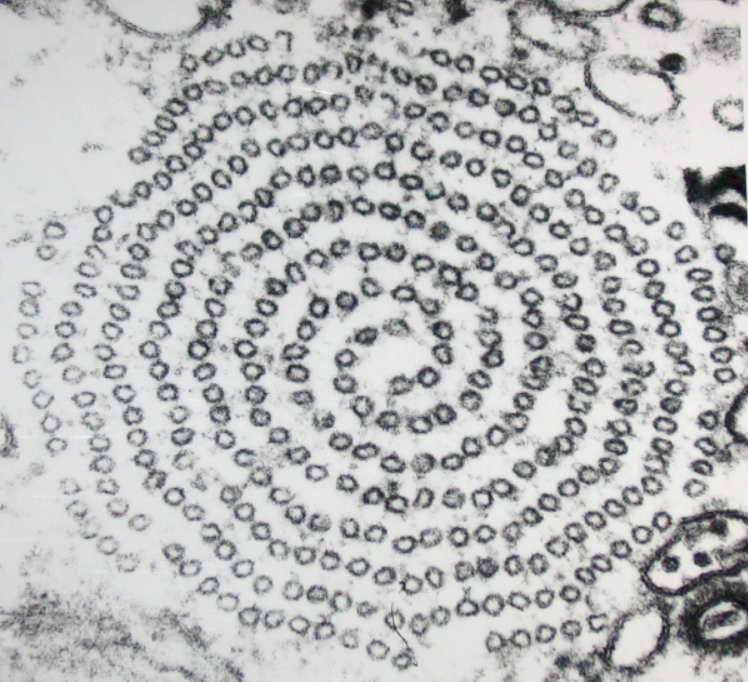
\includegraphics[width=\linewidth]{img/Axopodium_Mikrotubuli}
  \caption{Cross section of a Heliozoa's psuedopod, formed by a spiral structure of microtubules.}
  % https://de.wikipedia.org/wiki/Mikrotubulus#mediaviewer/File:Axopodium_Mikrotubuli.jpg
  \label{fig:microtubule}
\end{subfigure}\hfill
\begin{subfigure}{.31\linewidth}\centering
  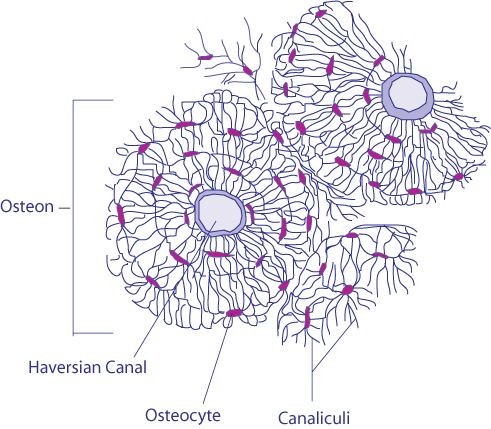
\includegraphics[width=\linewidth]{img/Transverse_Section_Of_Bone}
  \caption{Cross section of an osteon (the fundamental unit of compact bone) exhibiting its hierarchical structure.}
  % https://en.wikipedia.org/wiki/Osteon#mediaviewer/File:Transverse_Section_Of_Bone.png
  \label{fig:osteon}
\end{subfigure}\hfill
\begin{subfigure}{.31\linewidth}\centering
  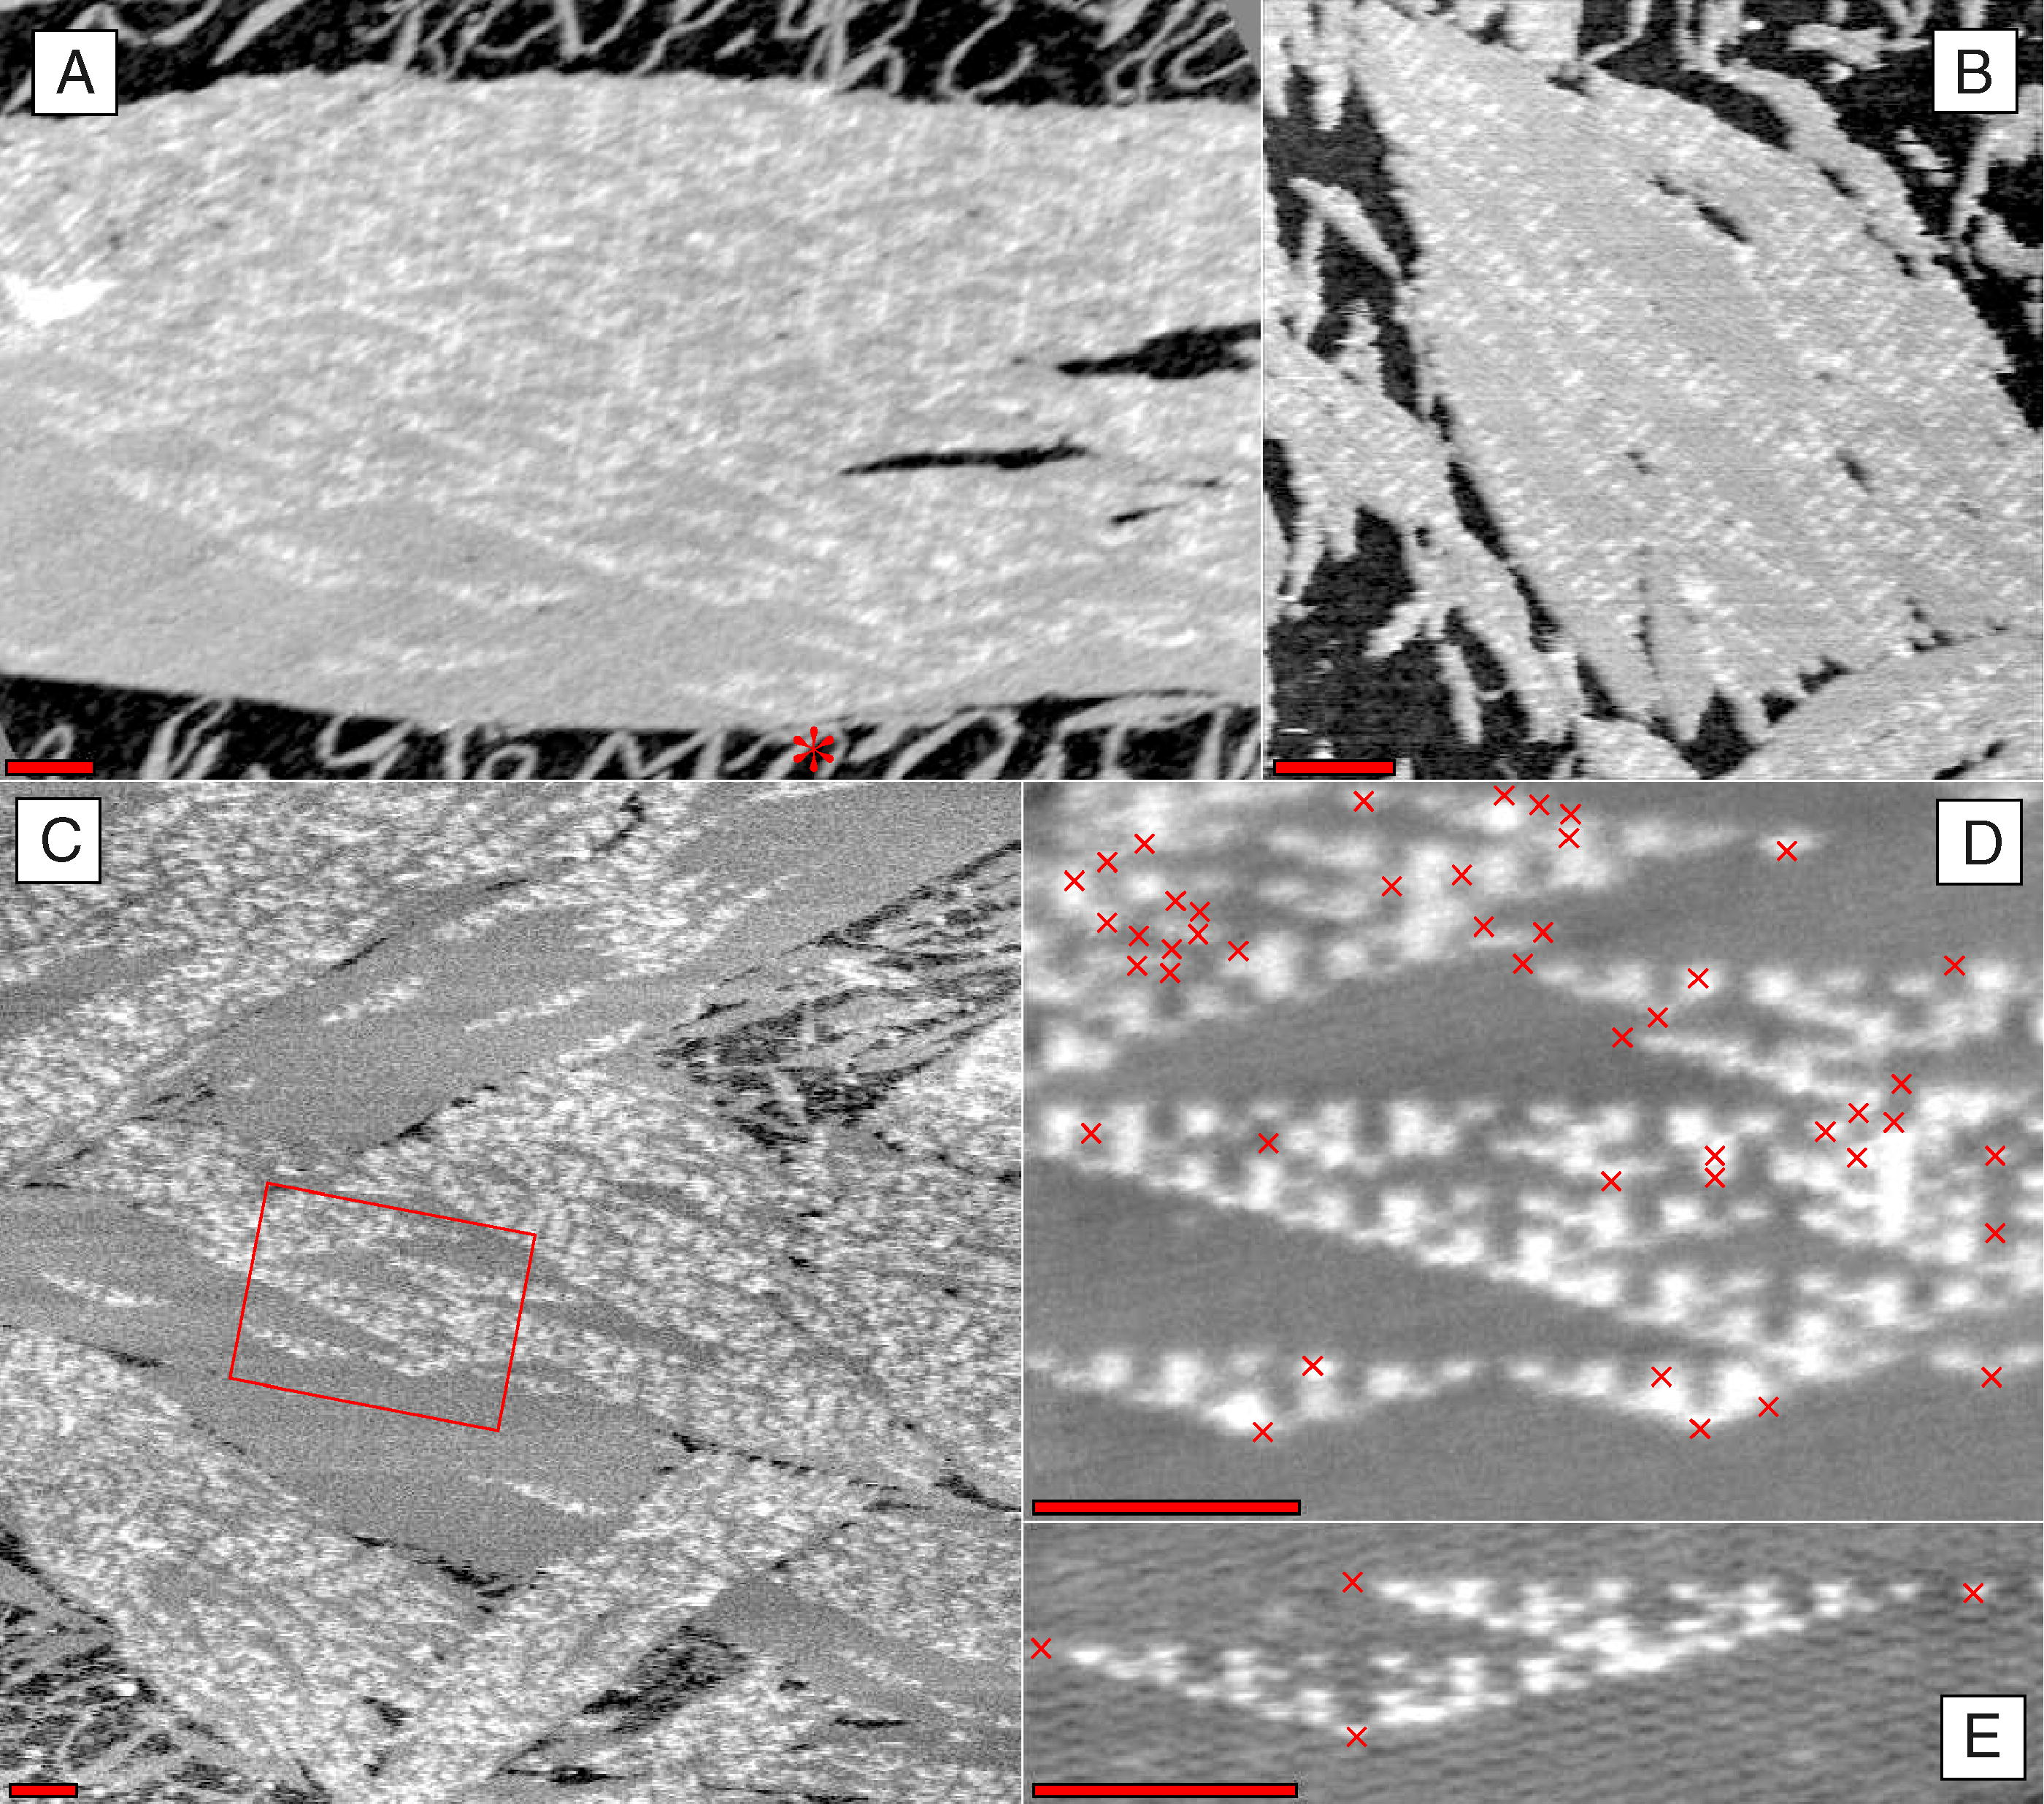
\includegraphics[width=\linewidth]{img/Rothemund-DNA-SierpinskiGasket}
  \caption{A DNA array exhibiting the Sierpinski triangle.}
  % https://en.wikipedia.org/wiki/DNA_nanotechnology#mediaviewer/File:Rothemund-DNA-SierpinskiGasket.jpg
  \label{fig:sierpinski}
\end{subfigure}
\caption{}
\end{figure*}


\begin{enumerate}
  %
    \item (cross-section) of microtubules \cite{Necklace1} e.g., in
ciliary membranes and transitions \cite{Necklace2}
   %
    \item (cross-section) of hierarchical bone structure \cite{XX} %
    \item crosslinked cellulose or collagen microfibril monolayers e.g.,
in cell-walls \cite{CellWalls1} \cite{CellWalls1}, as well as crosslinked
actin filaments in the cytoskeleton matrix.
  %
    \item more recent, engineered examples including  disordered graphene
layers \cite{Graphene1} \cite{Graphene2} sometimes reinforced
    by  microfibrils; and DNA assemblies \cite{Microfibrils1} including a
recent Sierpinski carpet, bringing other self-similar structures
    \cite{Microfibrils2} within reach.
    %
    \item  silica bi-layers, glass \cite{SilicaGlass1}
\cite{SilicaGlass2}, and materials that behave like assemblies of
    2D particles under non-overlap constraints, e.g, jammed
    disks on the plane \cite{JammedDisk1}
%
\end{enumerate}
%
In order to study structural and mechanical properties
such as rigidity, flexes and distribution of external stresses
within the material layer, it is natural to model a material
layer as a solution of a geometric constraint system
of appropriate types of geometric primitives, under
metric or algebraic constraints.
Such  2D {\bf{\em qusecs}} (quasi-uniform or self-similar
constraint systems) can be used to
understand or design material layers (their solutions)
with desired properties.
%
\subsection{Previous Work on Relevant 2D Geometric Constraint Systems} We
now briefly survey existing techniques for studying 2D {\em qusecs,}  many
of which are {\it bar-joint} systems (Examples 1,2 above, see Sections
\ref{sec:DRP}, \ref{sec:recomb}),
{\it multibody-pin} systems (Example 4,5, see Section \ref{sec:bodypin}) or  {\it
pinned-line incidence} systems (Example 3, see Section \ref{sec:pinnedline}). The
limitations of these techniques directly motivate
the contributions of this paper.

\medskip\noindent\underbar{{\sl (i) Finding (vertex)-maximal
generically rigid subsystems}}
Fast, graph-based algorithms exist (pebble-game \cite{XX}),
for locating all maximal, generically rigid subsystems \cite{XX}.
When the input is rigid, these algorithms compute the identity and  output
the input.

However, both for self-similar or just aperiodic 2D qusecs, it is
imperative to recursively decompose rigid systems
into their rigid subsystems, down to the level of
geometric primitives, in order to
understand or design properties at all scales, such as:
rigidity, flexes, distribution
of external stresses, boundary conditions for isostaticity,
as well as behavior under constraint variations.

\medskip\noindent\underbar{{\sl (ii) Optimal Recursive Decomposition
(DR-planning)}}
Recursive decomposition of geometric constraint systems has been
formalized \cite{XX} and well-studied \cite{XX}
as the {\sl Decomposition-Recombination (DR)-planning} problem.
For the above-mentioned classes of 2D qusecs, generic rigidity is
a combinatorial property and hence each level of the decomposition should,
in principle, be achievable by a graph-based algorithm as in (1), without
involving geometric information in the constraint system.
Since many  such decompositions can exist for a given constraint system,
criteria defining desirable or optimal DR-plans and DR-planning algorithms
were given in \cite{XX}. An {\em optimal DR-plan} is one
that minimizes the maximum number of child subsystems of any parent
system, a property that is
crucial for obtaining a solution to the parent constraint system from the
solutions of the child systems.

However, for general 2D qusecs, even when restricted to bar-joint systems,
the optimal DR-planning problem was shown to be NP-hard \cite{XX}.

\medskip\noindent\underbar{{\sl (iii) DR-plans for special classes and
with other criteria}}
For a special class of 2D qusecs, namely  {\em tree-decomposable} systems
\cite{XX} common in computer aided mechanical design,
(which includes ruler-and-compass and Henneberg-I constructible systems),
all DR-plans turn out to
be optimal. This satisfies the so-called {\em Church-Rosser} criterion,
leading to highly efficient DR-planning algorithms.
For general 2D qusecs, alternate criteria were suggested
such as {\em cluster minimality}
requiring parent systems to be composed of
a minimal set of at least 2 rigid proper subsystems (i.e., no proper
subset forms a rigid system);
and {\em proper maximality}, requiring child subsystems
to be maximal rigid proper subsystems of the parent system.

While polynomial time algorithms were given \cite{XX} to generate DR-plans
meeting the cluster minimality criterion,
no such algorithm is known for the latter criterion.


\medskip\noindent\underbar{{\sl (iv) Optimal Recombination and Solution
Space Navigation}}
For the entire DR-plan, finding all
desired solutions is barely tractable even if recombination
of solved subsystems is easy for each indecomposable parent system in the
DR-plan.
This is because even for the simplest, highly decomposable systems
with small DR-plans, the problem of finding even a single
solution to the input system at the root of the DR-plan
is NP-hard \cite{XX} and there is a
combinatorial explosion of solutions \cite{XX}. Typically, however,
the desired solution has a given orientation type, in which case,
the crux of the difficulty is concentrated in the algebraic complexity of
(re)combining child system solutions, to give a
solution to the parent system at any
given level of the DR-plan.
For fairly general 3D constraint systems,
there are algorithms with formal
guarantees that uncover underlying matroids to combinatorially
obtain an optimal parameterization to minimize the algebraic
complexity of the indecomposable parent (sub)systems that occur in the
DR-plan \cite{XX, XX,XX},
provided the DR-plan meets some of the abovementioned criteria.

However, the generality of these algorithms
trades-off against efficiency, and despite the optimization,
the best algorithms can still take
exponential time in the number of child subsystems (which can be arbitrarily
large even for optimal DR-plans) in order to guarantee
all solutions of a given orientation type,
even for a single (sub)system in a DR-plan. They
are prohibitively slow in practice. We note that utilizing the DR-plan and
optimal recombination as a principled basis, high performance heuristics
and software
exists \cite{XX,XX} to
tame combinatorial explosion via user intervention.


\medskip\noindent\underbar{{\sl (v) Configuration Spaces of
Underconstrained Systems}}
For underconstrained 2D bar-joint and multibody-pin cusecs obtained from
various subclasses of tree-decomposable systems, algorithms have been
developed \cite{XX, XX} that
to complete them into isostatic systems \cite{XX, XX} and to find paths
within the connected components \cite{XX,XX} of
standard cartesian configuration spaces. Most of the algorithms with
formal guarantees leverage Cayley configuration space theory \cite{XX,XX}
to characterize subclasses of graphs and additional constraints that
control combinatorial explosion, and provide faithful bijective
representation
of connected components and paths.
These algorithms have decreasing efficiency as the subclass of systems
gets bigger,  with highest efficiency for
underlying partial 2-tree graphs (alternately, tree-width 2,
series-parallel, $K_4$ minor avoiding),   moderate efficiency for
1 degree-of-freedom (dof) graphs with low Cayley complexity (which include
common linkages such as the Strandbeest, Limacon and Cardioid), and
decreased efficiency for general 1-dof tree-decomposable graphs. While
software suites exist \cite{XX,XX}, no such formal algorithms and
guarantees are known for non-tree-decomposable systems.
%
\subsection{Contributions and Organization}
\label{sec:cont}
The contributions of this paper are the following.
\begin{itemize}
\item
We  navigate the NP-hardness barrier mentioned in (2) above, for finding
optimal DR-plans by defining a
so-called {\it canonical} DR-plan and showing a strong Church-Rosser
property: {\it all canonical DR-plans for isostatic or
underconstrained
2D qusecs are optimal} (Section \ref{sec:DRP}).
\item
We give an efficient ($O(n^2)$) algorithm to find a canonical (and hence
optimal) DR-plan for all 3 types of 2D qusecs mentioned above (Sections
\ref{sec:DRP}, \ref{sec:bodypin}, and \ref{sec:pinnedline}.
The canonical DR-plan
illuminates the essence of the NP-hardness of finding optimal DR-plans for
overconstrained systems.
\item
We give a method to deal with the
algebraic complexity of recombining the realizations or
solutions of  child subsystems into a solution of the parent system.
Specifically, we define the problem of  minimally modifying the
indecomposable recombination system so that it becomes decomposable via a
 small DR-plan and yet preserves the original
solutions in an efficiently searchable manner. We show formal connection
to well known problems such as optimal completion of
underconstrained  systems  \cite{XX}.  When the required modifications
are bounded, we obtain new, efficient algorithms for
realizing both isostatic and underconstrained
qusecs by leveraging recent results about Cayley parameters in
\cite{XX,XX}  (Section \ref{sec:recomb}).
\item
We briefly describe applications of the above techniques to modeling,
analyzing and designing specific properties in 2D material layers.
For Examples 1,2 (achieving isostaticity, distribution of stresses in
self-similar, bar-joint systems); Example 3 (canonical and optimal
DR-plans for pinned line incidence systems \cite{XX}) and Examples 4,5
(boundary-conditions for achieving various desired properties
of multi-body  pin systems).

\item
Software implementation and videos can be found at: \todo{Provide Link}.
\end{itemize}


\section{Preliminaries and Background}
\label{sec:prelim}

% Basics definitions and theory for this topic can be found in~\ref{sec:appendix:defs}.

We first give basic definitions and concepts in combinatorial rigidity, leading to a definition of a DR-plan, its properties, and how they relate. The section ends with a discussion of previous work on DR-plans.

\subsection{Geometric Constraint Systems and Combinatorial Rigidity}
\label{sec:prelim:defs}
\label{sec:appendix:defs}


In this paper, a \dfn{geometric constraint system} is a multivariate polynomial (usually bilinear or quadratic) system $G(x,\delta)=0$, representing constraints with parameters $\delta$ between geometric primitives  in $\mathbb{R}^2$ represented collectively as $x\in \mathbb{R}^n$.
%
When the type of constraint (system) is fixed, the system is simply represented as $(G,\delta)$, where $G$ is the underlying constraint (hyper)graph $G = (V,E)$ with the vertices $V$ representing the geometric primitives in $\mathbb{R}^2$ and (hyper)edges $E$ representing the constraints, each with an associated parameter $\delta$.
%
For example, a \dfn{bar-joint system or linkage} $(G,\delta)$, is a graph $G=(V,E)$ with fixed length bars as edges,
% \footnote{Geometric constraint systems can also have inequalities in addition to equations, where the parameters in $\delta$ are small intervals of values rather than exact values.}
i.e.\ $\delta: E \rightarrow \mathbb{R}$; this represents the distance constraint system $\| x_u -x_v \|_2 = \delta_{u,v}$ for  $(u,v) \in E$, where $x_u \in \mathbb{R}^2$ represents the coordinates of $u\in V$.



In all types of geometric constraint systems we consider in this paper, a Cartesian \dfn{realization} or \dfn{solution} $G(p)$ of $(G,\delta)$ is an assignment of coordinates or Euclidean transformations (poses), $p: V \rightarrow \mathbb{R}^2$ or $\mathbb{R}^3$, to the vertices of $G$ satisfying the constraints with parameters $\delta$, modulo orientation preserving isometries (Euclidean rigid body motions).

Although the realization space itself depends on the constraint parameters $\delta$, many relevant \dfn{generic} properties of the constraint system $G(x,\delta)$ are defined to be properties of the constraint (hyper)graph $G$ and do not depend on $\delta$ (or they hold for all but a measure zero set of $\delta$ values). Many of these are properties of the Jacobian $\Delta_x G(x,\delta)$, often called the appropriate \dfn{rigidity matrix of $G$} (a matrix of indeterminates). For example, the \dfn{bar-joint rigidity matrix of the graph $G = (V,E)$} is a matrix of indeterminates representing the Jacobian of the distance map $\| x_u -x_v \|_2$  for $(u,v) \in E$. The matrix has $2$ columns per vertex in $V$ and one row per edge in $E$, where the row corresponding to edge $(u,v)$ contains the 2 coordinate indeterminates for $x_u -x_v$ (resp. $x_v-x_u$) in the 2 columns for $u$ (resp.\ $v$), i.e.\ 4 non-zero entries per row.


% XXXXXXXXX
% something has to be said along with asimow roth
% (infinitesimal rigidity implies rigidity) When the rigidity matrix has
% appropriate rank, the realizations or solutions of the corresponding
% constraint system are generically isolated and zero-dimensional if the
% constraint system has equalities and exact values for the parameters
% $\delta$. If the constraint system has inequalities, i.e, if the
% $\delta$ lie in an interval, this claim is approximate: the solutions
% are isolated small, full-dimensional  connected components.

One important property of a generic constraint system or (hyper)graph\footnote{We refer to these as properties of the constraint system or as properties of the underlying (hyper)graph interchangeably}
%that depends on the appropriate rigidity matrix of indeterminates
is \dfn{rigidity},
% (\note footnote now...),
i.e.\ the realizations or solutions of the corresponding constraint system being generically isolated and zero-dimensional.
%(if the constraint system has equalities and exact values for the parameters $\delta$).
The result by Asimow and Roth \cite{asimow1978rigidity}  shows a constraint (hyper)graph is rigid if and only if  it is generically \dfn{infinitesimally rigid}, i.e.\ the number of independent rows of its appropriate rigidity matrix is at least the number of columns less the number of rigid body motions, which is 3 for 2D bar-joint systems.
%This condition is called generic {\em infinitesimal rigidity}.

% \sidenote{If the constraint system has inequalities, i.e, if the $\delta$ lie in an interval, the definition of rigidity is approximate: the solutions are isolated small, full-dimensional  connected components.}
% generic rigidity, i.e.\ there exist at most finitely many solutions to the system at generic points,  %to the algebraic system

Geometric constraint systems can also have inequalities in addition to equations, where the parameters in $\delta$ are small intervals rather than exact values. In this case, the definition of rigidity is approximate; the solutions are isolated, small, full-dimensional connected components.

Other generic constraint system or (hyper)graph properties are mentioned here.
% (\note we refer to these as properties of the constraint
% system or as properties of the underlying (hyper)graph
% interchangeably).
A constraint (hyper)graph $G$ is \dfn{independent} if its appropriate rigidity matrix of indeterminates has independent rows (i.e.\ the determinant of some square submatrix is not identically zero).
%It is {\em rigid} if the number of independent rows of the rigidity matrix is
%at least the number of columns less the number of rigid body motions,
%which is 3 for distance constraint systems.
It is \dfn{isostatic} (\dfn{minimally rigid}, \dfn{wellconstrained}) if it is both rigid and independent.
%if the number of generically independent rows or the rank of the appropriate rigidity matrix is maximal.
%For example, the maximal rank of a bar-joint rigidity matrix is $2|V| - 3$,
%where $3$ is the number of rotational and translational degrees-of-freedom of a rigid body in $\mathbb{R}^2$.
%The graph $G$ is {\em rigid} if there exists some spanning subgraph $S\subseteq G$ such that $S$ is wellconstrained.
It is \dfn{flexible} if it is not rigid, \dfn{underconstrained} if it is independent and not rigid, or \dfn{overconstrained} if it is not independent.

Defining the combinatorial independence of a subset of edges $E'\subseteq E$ to be the independence of corresponding rows in the rigidity matrix of indeterminates, we obtain the \dfn{rigidity matroid} of a constraint (hyper)graph $G = (V,E)$.
%The 2-dimensional {\em rigidity matroid} of a constraint (hyper)graph $G = (V,E)$ is a linear matroid  on $E$,
%where a subset of edges $E' \subseteq E$ is {\em independent} in the matroid,
%if the set of corresponding rows in the appropriate rigidity matrix of indeterminates are linearly independent.
There are various results on combinatorial characterization of independence, rigidity, and rigidity matroids for different types of (hyper)graphs. For bar-joint rigidity matroids, the famous Laman's theorem \cite{laman1970graphs} states that the underlying graph is isostatic if and only if $|E| = 2|V|-3$ and $|E'| \le 2|V'|-3$ for every induced subgraph with at least 2 vertices. The result by Lovasz and Yemini \cite{lovasz1982generic} shows that all 6-vertex-connected graphs are rigid in the plane. For bar-body rigidity matroids, Tay \cite{tay1976rigidity} proved that the underlying multigraph is isostatic if and only if it can be decomposed as $3$ edge disjoint spanning trees. White and Whiteley \cite{white1987algebraic} gave the same characterization using a different technique to study the algebraic-geometric conditions of genericity, called pure condition. Lee, Streinu and Theran \cite{lee2007graded} defined the \dfn{$(k,l)$-sparsity matroid}, where a hypergraph $G$ is called \dfn{$(k,l)$-sparse} if $|E'| \le k|V'| - l$ for any induced subgraph $(V',E')$ with at least 2 vertices, and \dfn{$(k,l)$-tight} if it is $(k,l)$-sparse and $|E| = k|V| - l$. In general, given a $d$-uniform hypergraph, a $(k,l)$-sparsity condition is matroidal as long as $l \le dk-1$.

In this paper, a \dfn{qusecs} is any independent geometric constraint system of one of 3 types: bar-joint (defined formally in \ref{sec:prelim:defs}), \dfn{body-hyperpin} (defined formally in Section \ref{sec:bodypin}), and \dfn{pinned line-incidence} (defined formally in Section \ref{sec:pinnedline}).



% In this paper, a \dfn{qusecs} is any \dfn{independent} geometric constraint system of one of the 3 types mentioned above.

% % \medskip\noindent
% % \note In the remainder of this section and sections~\ref{sec:DRP} and \ref{sec:recomb} we only consider bar-joint qusecs and graphs. Relevant formal analogies for the other 2 types of qusecs and (hyper)graphs are given in the subsequent 2 sections on Applications.

% \sidenote{In the remainder of this section and Sections~\ref{sec:DRP} and \ref{sec:recomb} we only consider bar-joint qusecs and graphs. Relevant formal analogies for the other 2 types of qusecs and (hyper)graphs are given in the subsequent 2 sections on Applications (\ref{sec:bodypin} and \ref{sec:pinnedline}).}



%XXXNow comes the definition of stress vector and flex vector.
%NOTE: something has to be said about what flexes and stresses mean


%TODO
%Given a bar-joint graph, a vector (of indeterminates) in the right null space of its rigidity matrix is called a \dfn{flex vector}. It has 2 entries per vertex and represents the internal motions of the system (i.e.\ modulo rigid body motions). For rigid graphs, all flex vectors are identically zero.
%
%A vector (of indeterminates) in the left null space of the rigidity matrix is called a \dfn{stress vector}. It has one entry per edge and represents a \dfn{self stress} of the system. For independent graphs, all stress vectors are identically zero.
%
%An \dfn{external stress} $t$ is a $1\times 2|V|$ vector  (of indeterminates) which specifies a 2D vector acting at each vertex such that the stress balance equation $sR = t$ holds, where $s$ is a vector of internal stresses, one for each bar, and $R$ is the rigidity matrix.




%\subsection{Qusecs}


% \medskip\noindent
% \note In the remainder of this section and sections~\ref{sec:DRP} and \ref{sec:recomb} we only consider bar-joint qusecs and graphs. Relevant formal analogies for the other 2 types of qusecs and (hyper)graphs are given in the subsequent 2 sections on Applications.

We note that  the remainder of this section and Sections~\ref{sec:DRP} and \ref{sec:recomb} we only consider bar-joint qusecs and graphs. Relevant formal analogies for the other 2 types of qusecs and (hyper)graphs are given along with their materials applications in Sections \ref{sec:bodypin} and \ref{sec:pinnedline}.






\subsection{Decomposition-Recombination (DR-) Plans}
%
%$G=(V,E,w_V,w_E)$ is a set of vertices, $V$, and a set of edges, $E$, defined as a tuple of vertices from $V$ (undirected). Additionally, there are two weight functions, $w_V: V \to \mathbb{R}^+$ and $w_E: E \to \mathbb{R}^+$. The \textbf{density} of graph $G$ is $d(G) = \sum_{e\in E}{w_E(e)} - \sum_{v\in V}{w_V(v)}$.
%
%Given a constant $k$, a graph $G$ is:
%\begin{itemize}
%    \item \textbf{independent} (or \textbf{sparse}) if, for all non-trivial subgraphs $S\subseteq G$, $d(S) \leq k$.
%
%    \item \textbf{overconstrained} if it is not independent.
%
%    \item \textbf{wellconstrained} (or \textbf{tight}) if $G$ is independent and $d(G)=k$.
%
%    \item \textbf{rigid} if there exists some spanning subgraph $S\subseteq G$ such that $S$ is wellconstrained.
%
%    \item \textbf{underconstrained} if $G$ is independent and not rigid.
%
%    % \item \textbf{trivial} if (1) it is overconstrained graph and (2) all of its subgraphs are also trivial. Trivial graphs are input.
%\end{itemize}
%
% \begin{definition}
%     A graph is \textbf{overconstrained} if, given constant $k$, there exists some
%     % induced
%     subgraph $S\subseteq G$ such that $d(S) > k$.
% \end{definition}
%
% \begin{definition}
%     A graph is \textbf{wellconstrained} if, given constant $k$, $d(G) = k$ and for all
%     % induced
%     subgraphs $S\subseteq G$, (1) $d(S)\leq k$, or (2) given a set of trivial graphs $T$, $S$ is isomorphic to one of the graphs in $T$ (i.e.\ $S$ is trivial).
% \end{definition}
%
%
%
% \begin{definition}
%     A \textbf{trivial} graph is ill-defined in the general case. The only strict requirements are: (1) it must be an overconstrained graph and (2) all of its subgraphs are also trivial.
%     \todo{Maybe leave the following out until it's needed later?}
%     In the familiar geometric cases of $d$-dimensional space, all vertex weights are $d$, all edge weights are $1$, and constant $k= -{{d+1}\choose{2}}$. Trivial graphs for 2D would be a single vertex. Trivial graphs in 3D would be a vertex and an edge (2 vertices with an edge between). Etc. These trivial graphs capture the notion of the rotational symmetry that exists in geometric spaces.
% \end{definition}
%


% \ClearMyMinHeight
% \SetMyMinHeight{.4}{../../img/epsfromtikz/demo_graph}
% \SetMyMinHeight{.3}{../../img/epsfromtikz/demo_graph_comdrp}
% \SetMyMinHeight{.3}{../../img/epsfromtikz/demo_graph_candrp}

% \begin{figure*}\centering%
%   %
%   \begin{subfigure}{0.4\linewidth}\centering
%     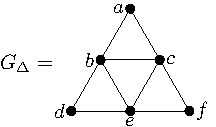
\includegraphics[height=\myMinHeight]{../../img/epsfromtikz/demo_graph}
%     \caption{}\label{fig:demo_graph:graph}
%   \end{subfigure}%
%   %
%   \hfill
%   \begin{subfigure}{0.3\linewidth}\centering
%     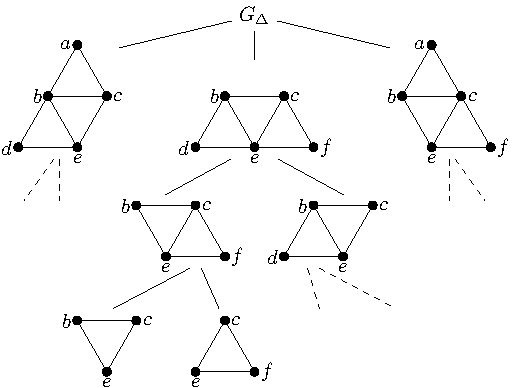
\includegraphics[height=\myMinHeight]{../../img/epsfromtikz/demo_graph_comdrp}
%     \caption{}\label{fig:demo_graph:comdrp}
%   \end{subfigure}%
%   %
%   \hfill
%   \begin{subfigure}{0.3\linewidth}\centering
%     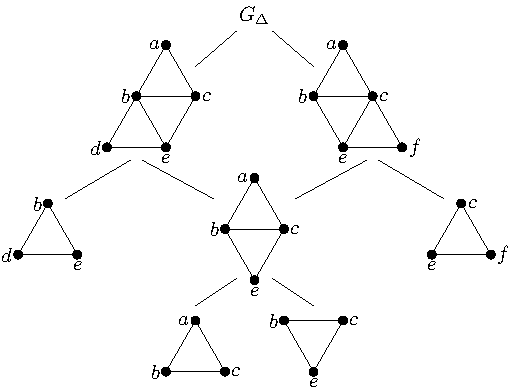
\includegraphics[height=\myMinHeight]{../../img/epsfromtikz/demo_graph_candrp}
%     \caption{}\label{fig:demo_graph:candrp}
%   \end{subfigure}%
%   %
%   \caption{(\ref{fig:demo_graph:graph}) A simple graph, $G_{\Delta}$, used to illustrate concepts throughout this and the next section. (\ref{fig:demo_graph:comdrp}) The complete DR-plan of $G_{\Delta}$, i.e.\ $ComDRP(G_{\Delta})$. Dashed lines indicate that the children repeat the same pattern as the others shown on this level. The children of triangles (3 edges) are omitted. (\ref{fig:demo_graph:candrp}) The canonical DR-plan of $G_{\Delta}$, which is optimal (see Section~\ref{sec:DRP}), i.e.\ $OptDRP(G_{\Delta})$. The children of triangles are omitted.}
%   \label{fig:demo_graph}
% \end{figure*}%



% \begin{figure*}\centering%
%   %
%   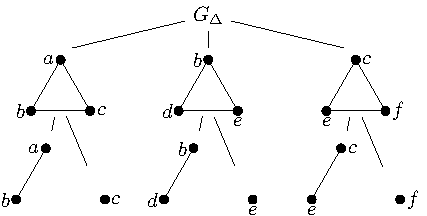
\includegraphics[width=0.4\linewidth]{../../img/epsfromtikz/demo_graph_clustmindrp}
%   \caption{A DR-plan of $G_{\Delta}$ from Figure~\ref{fig:demo_graph:graph}, which gives cluster minimality. Using the ideas from the paper~\cite{lomonosov2004graph}, the children of a triangle are the primitives of a point and an edge. Thus, the fan-in of this graph is 3, whereas the optimal DR-plans shown in Figure~\ref{fig:demo_graph:candrp} and \ref{fig:demo_graph:candrpseq} have fan-in of 2. With this counterexample, it is clear that cluster minimality is not sufficient for optimality.}
%   \label{fig:demo_graph:clustmindrp}
% \end{figure*}%



\ClearMyMinHeight
\SetMyMinHeight{.4}{../../img/svg/3xc2c3_new}
\SetMyMinHeight{.3}{../../img/svg/3xc2c3_new_comdrp}
\SetMyMinHeight{.3}{../../img/svg/3xc2c3_new_candrp}

\begin{figure*}\centering%

  \begin{subfigure}{0.4\linewidth}\centering
    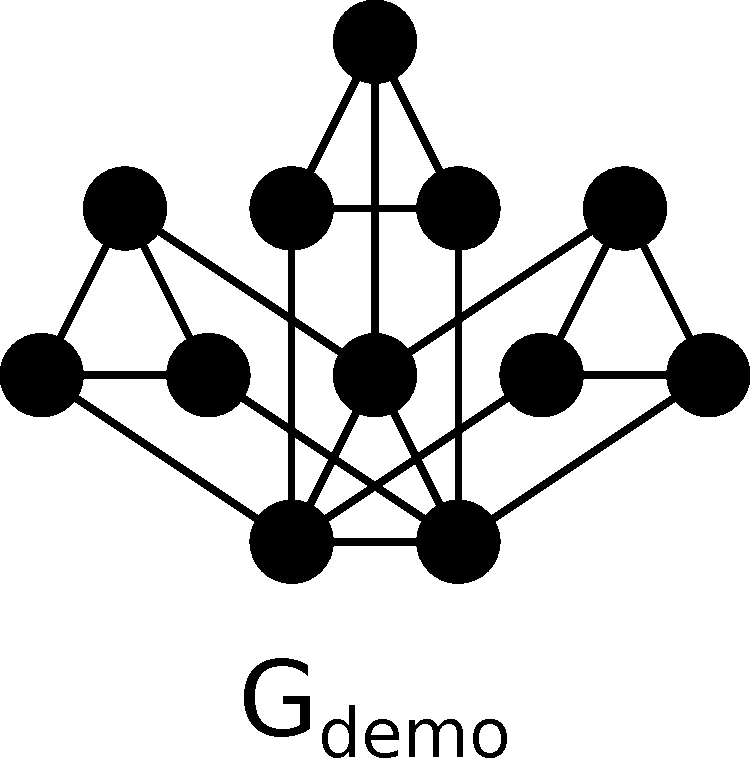
\includegraphics[height=\myMinHeight]{../../img/svg/3xc2c3_new}
    \caption{}\label{fig:demo_graph:graph}
  \end{subfigure}%
  %
  \hfill
  \begin{subfigure}{0.3\linewidth}\centering
    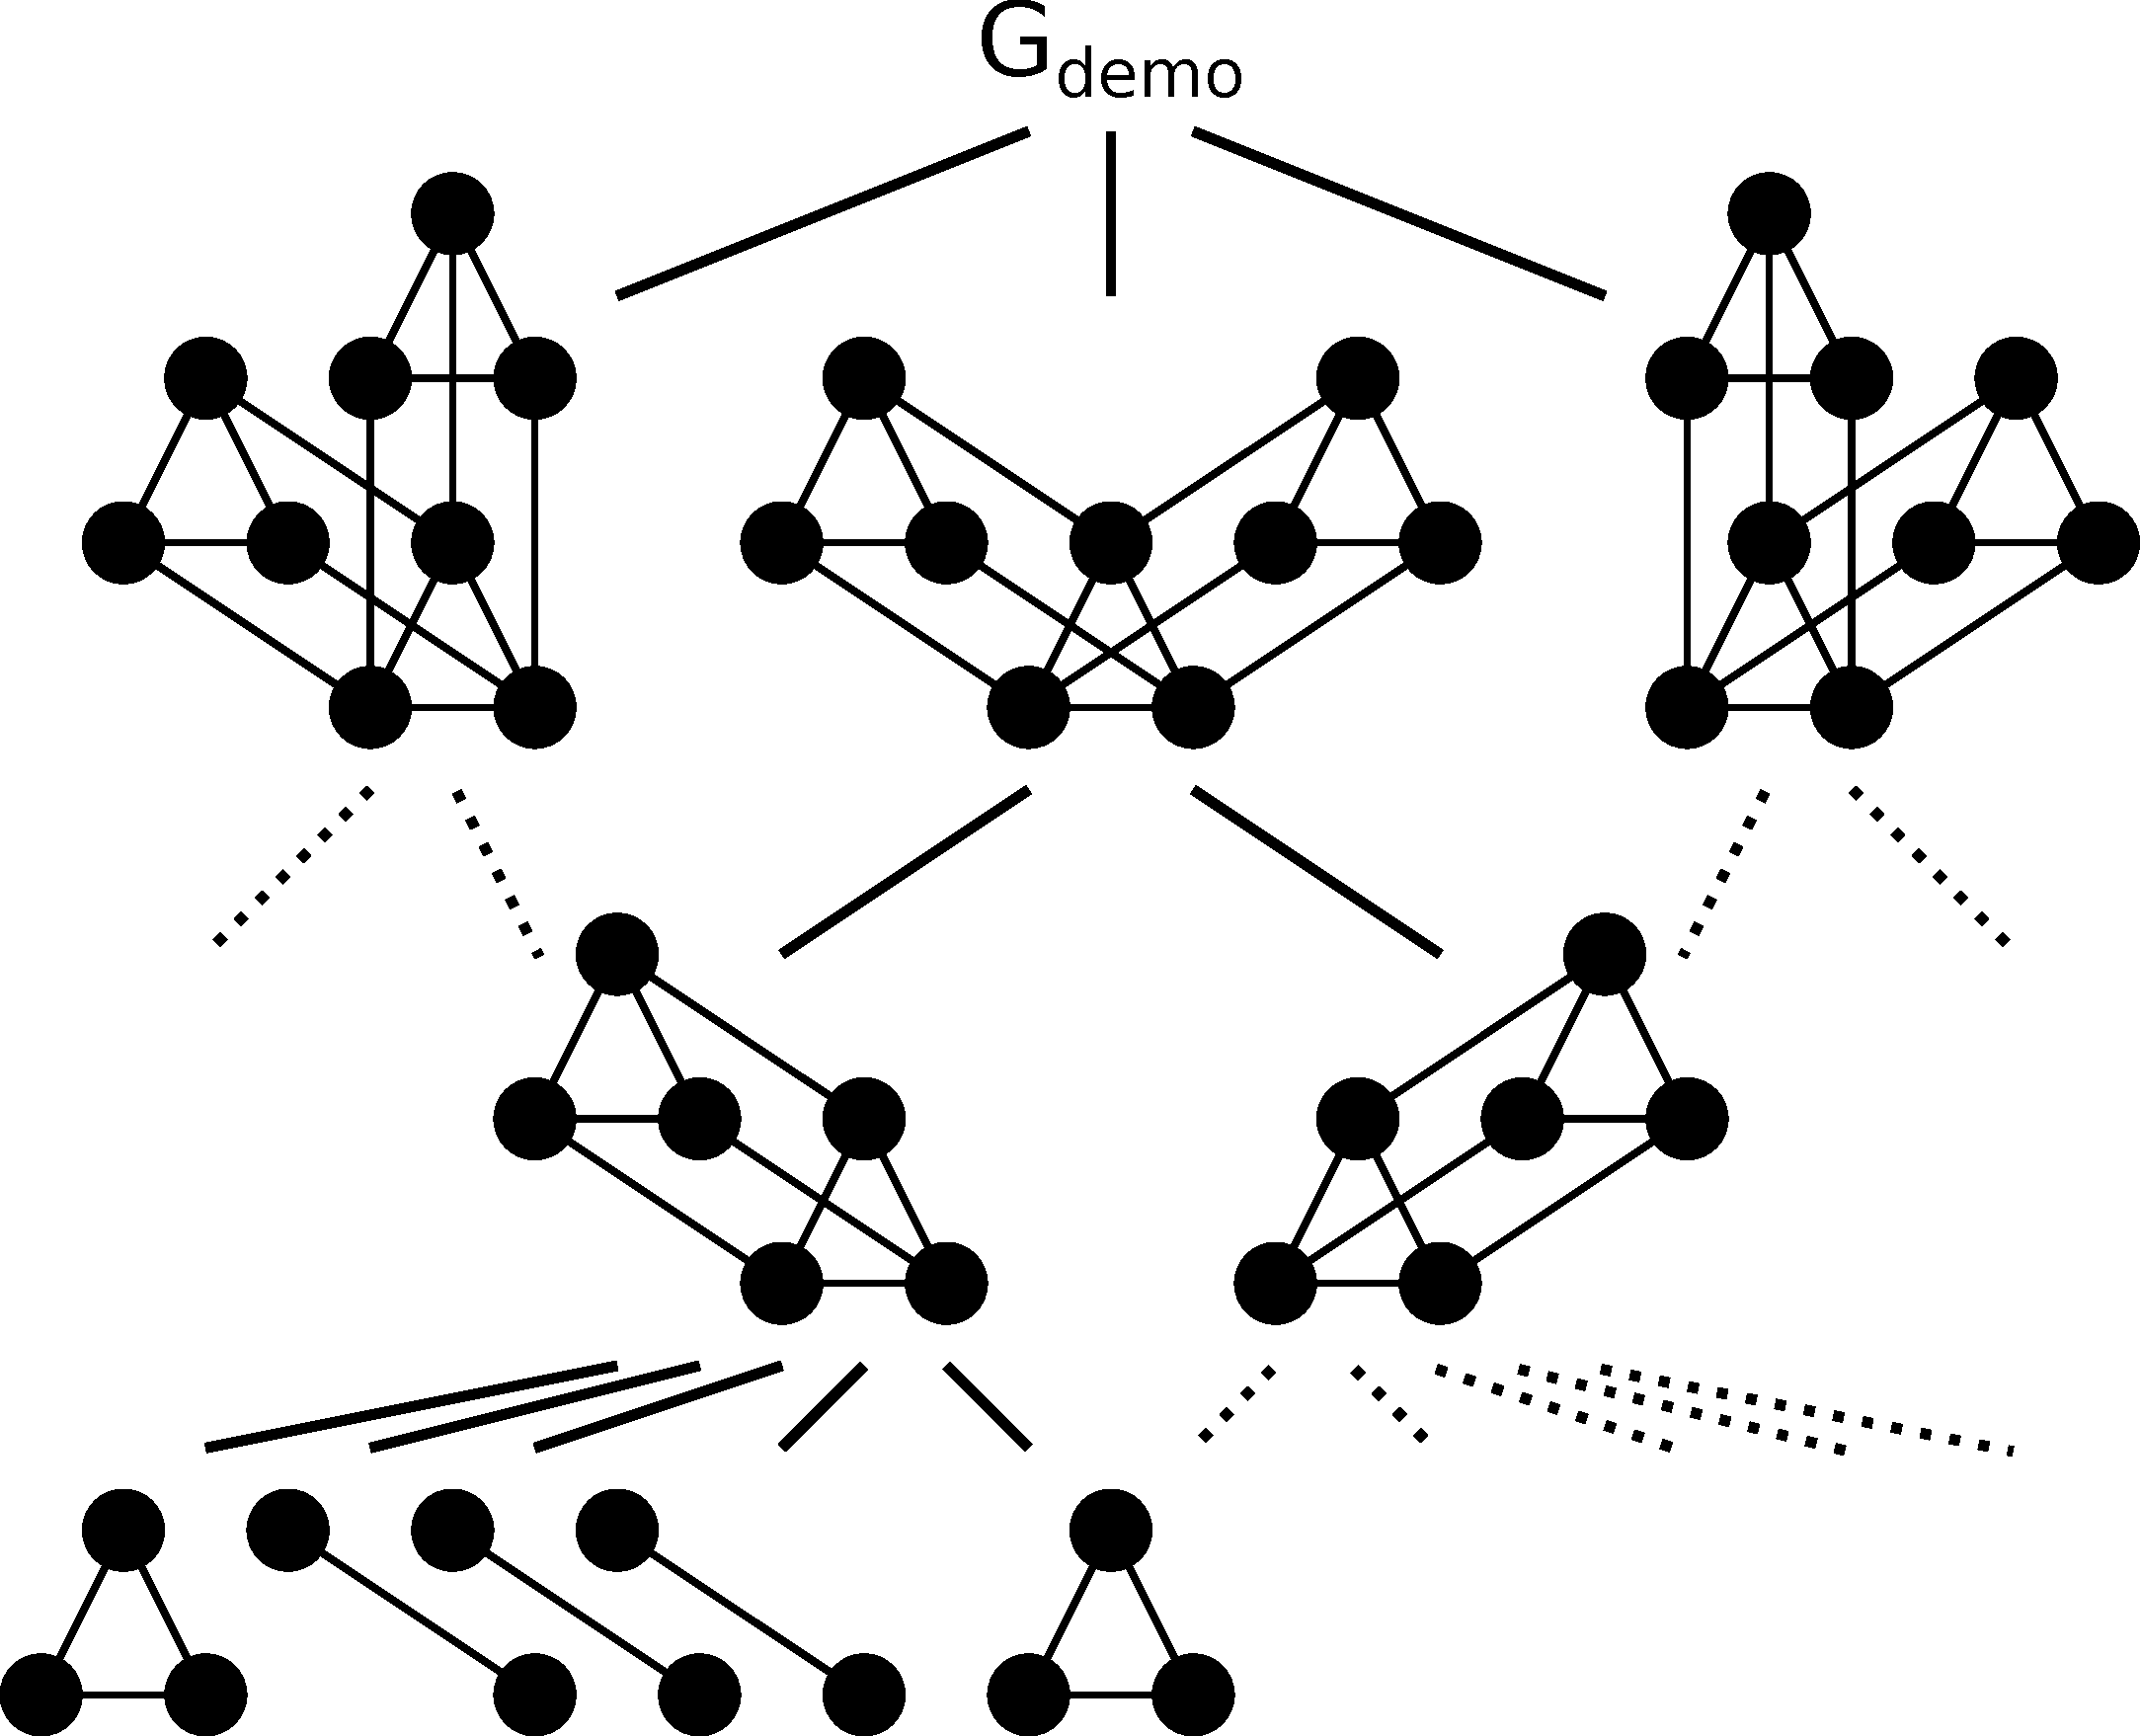
\includegraphics[height=\myMinHeight]{../../img/svg/3xc2c3_new_comdrp}
    \caption{}\label{fig:demo_graph:comdrp}
  \end{subfigure}%
  %
  \hfill
  \begin{subfigure}{0.3\linewidth}\centering
    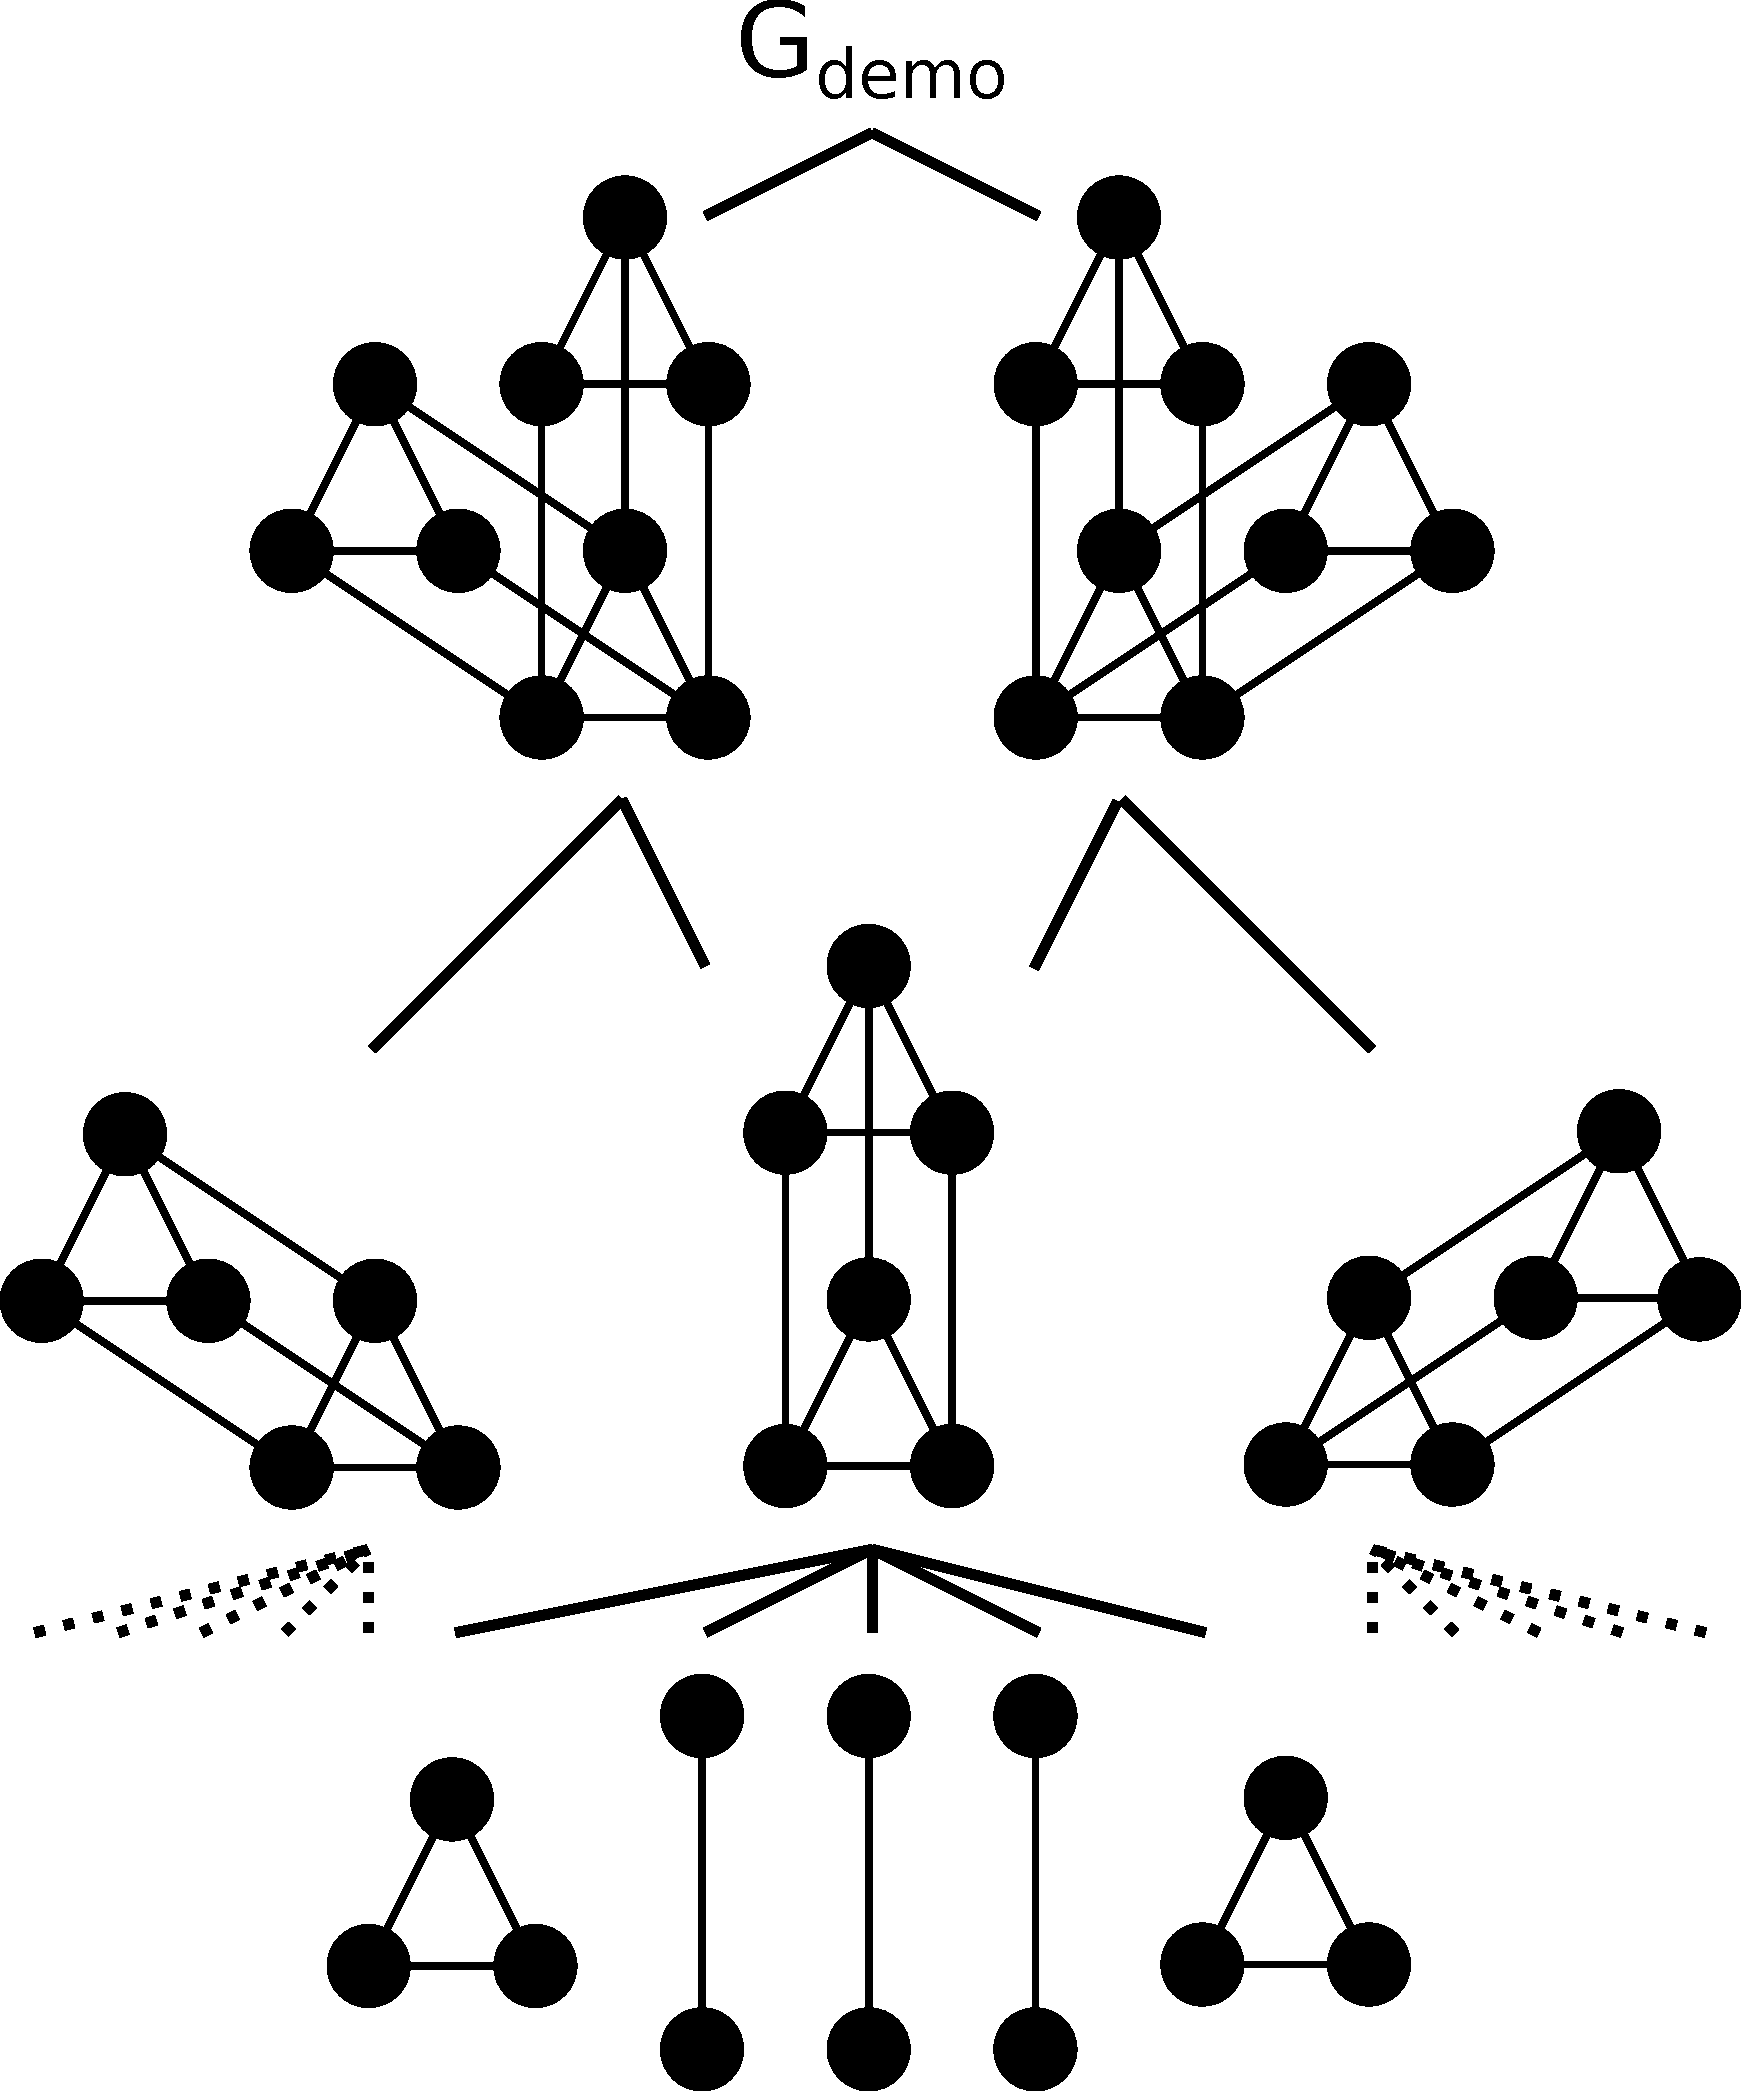
\includegraphics[height=\myMinHeight]{../../img/svg/3xc2c3_new_candrp}
    \caption{}\label{fig:demo_graph:candrp}
  \end{subfigure}%
  %
  % \begin{subfigure}[c]{0.3\linewidth}\centering
  %   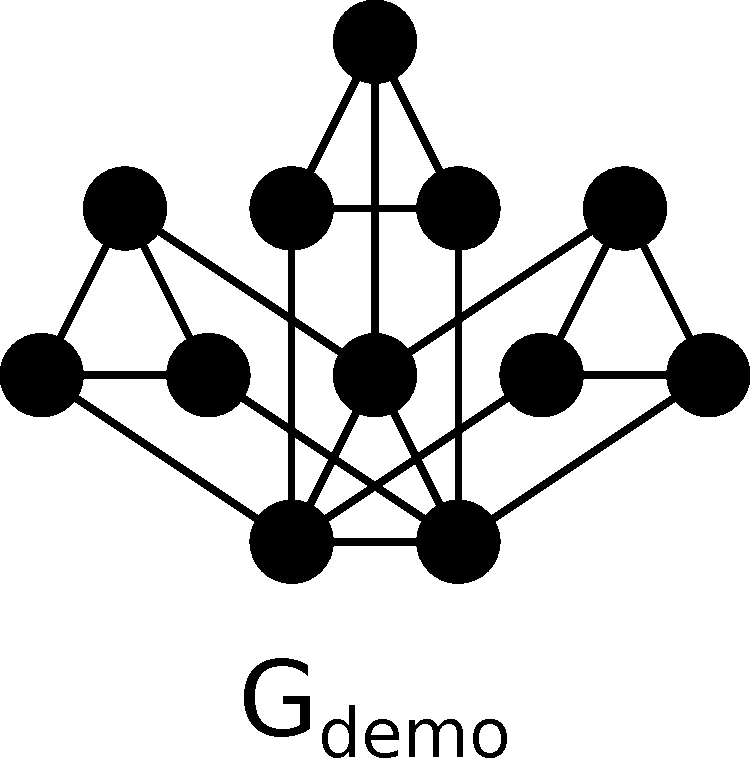
\includegraphics[width=\linewidth]{../../img/svg/3xc2c3_new}
  %   \caption{}\label{fig:demo_graph:graph}
  % \end{subfigure}%
  % %
  % \hfill
  % \begin{subfigure}[t]{0.345\linewidth}\centering
  %   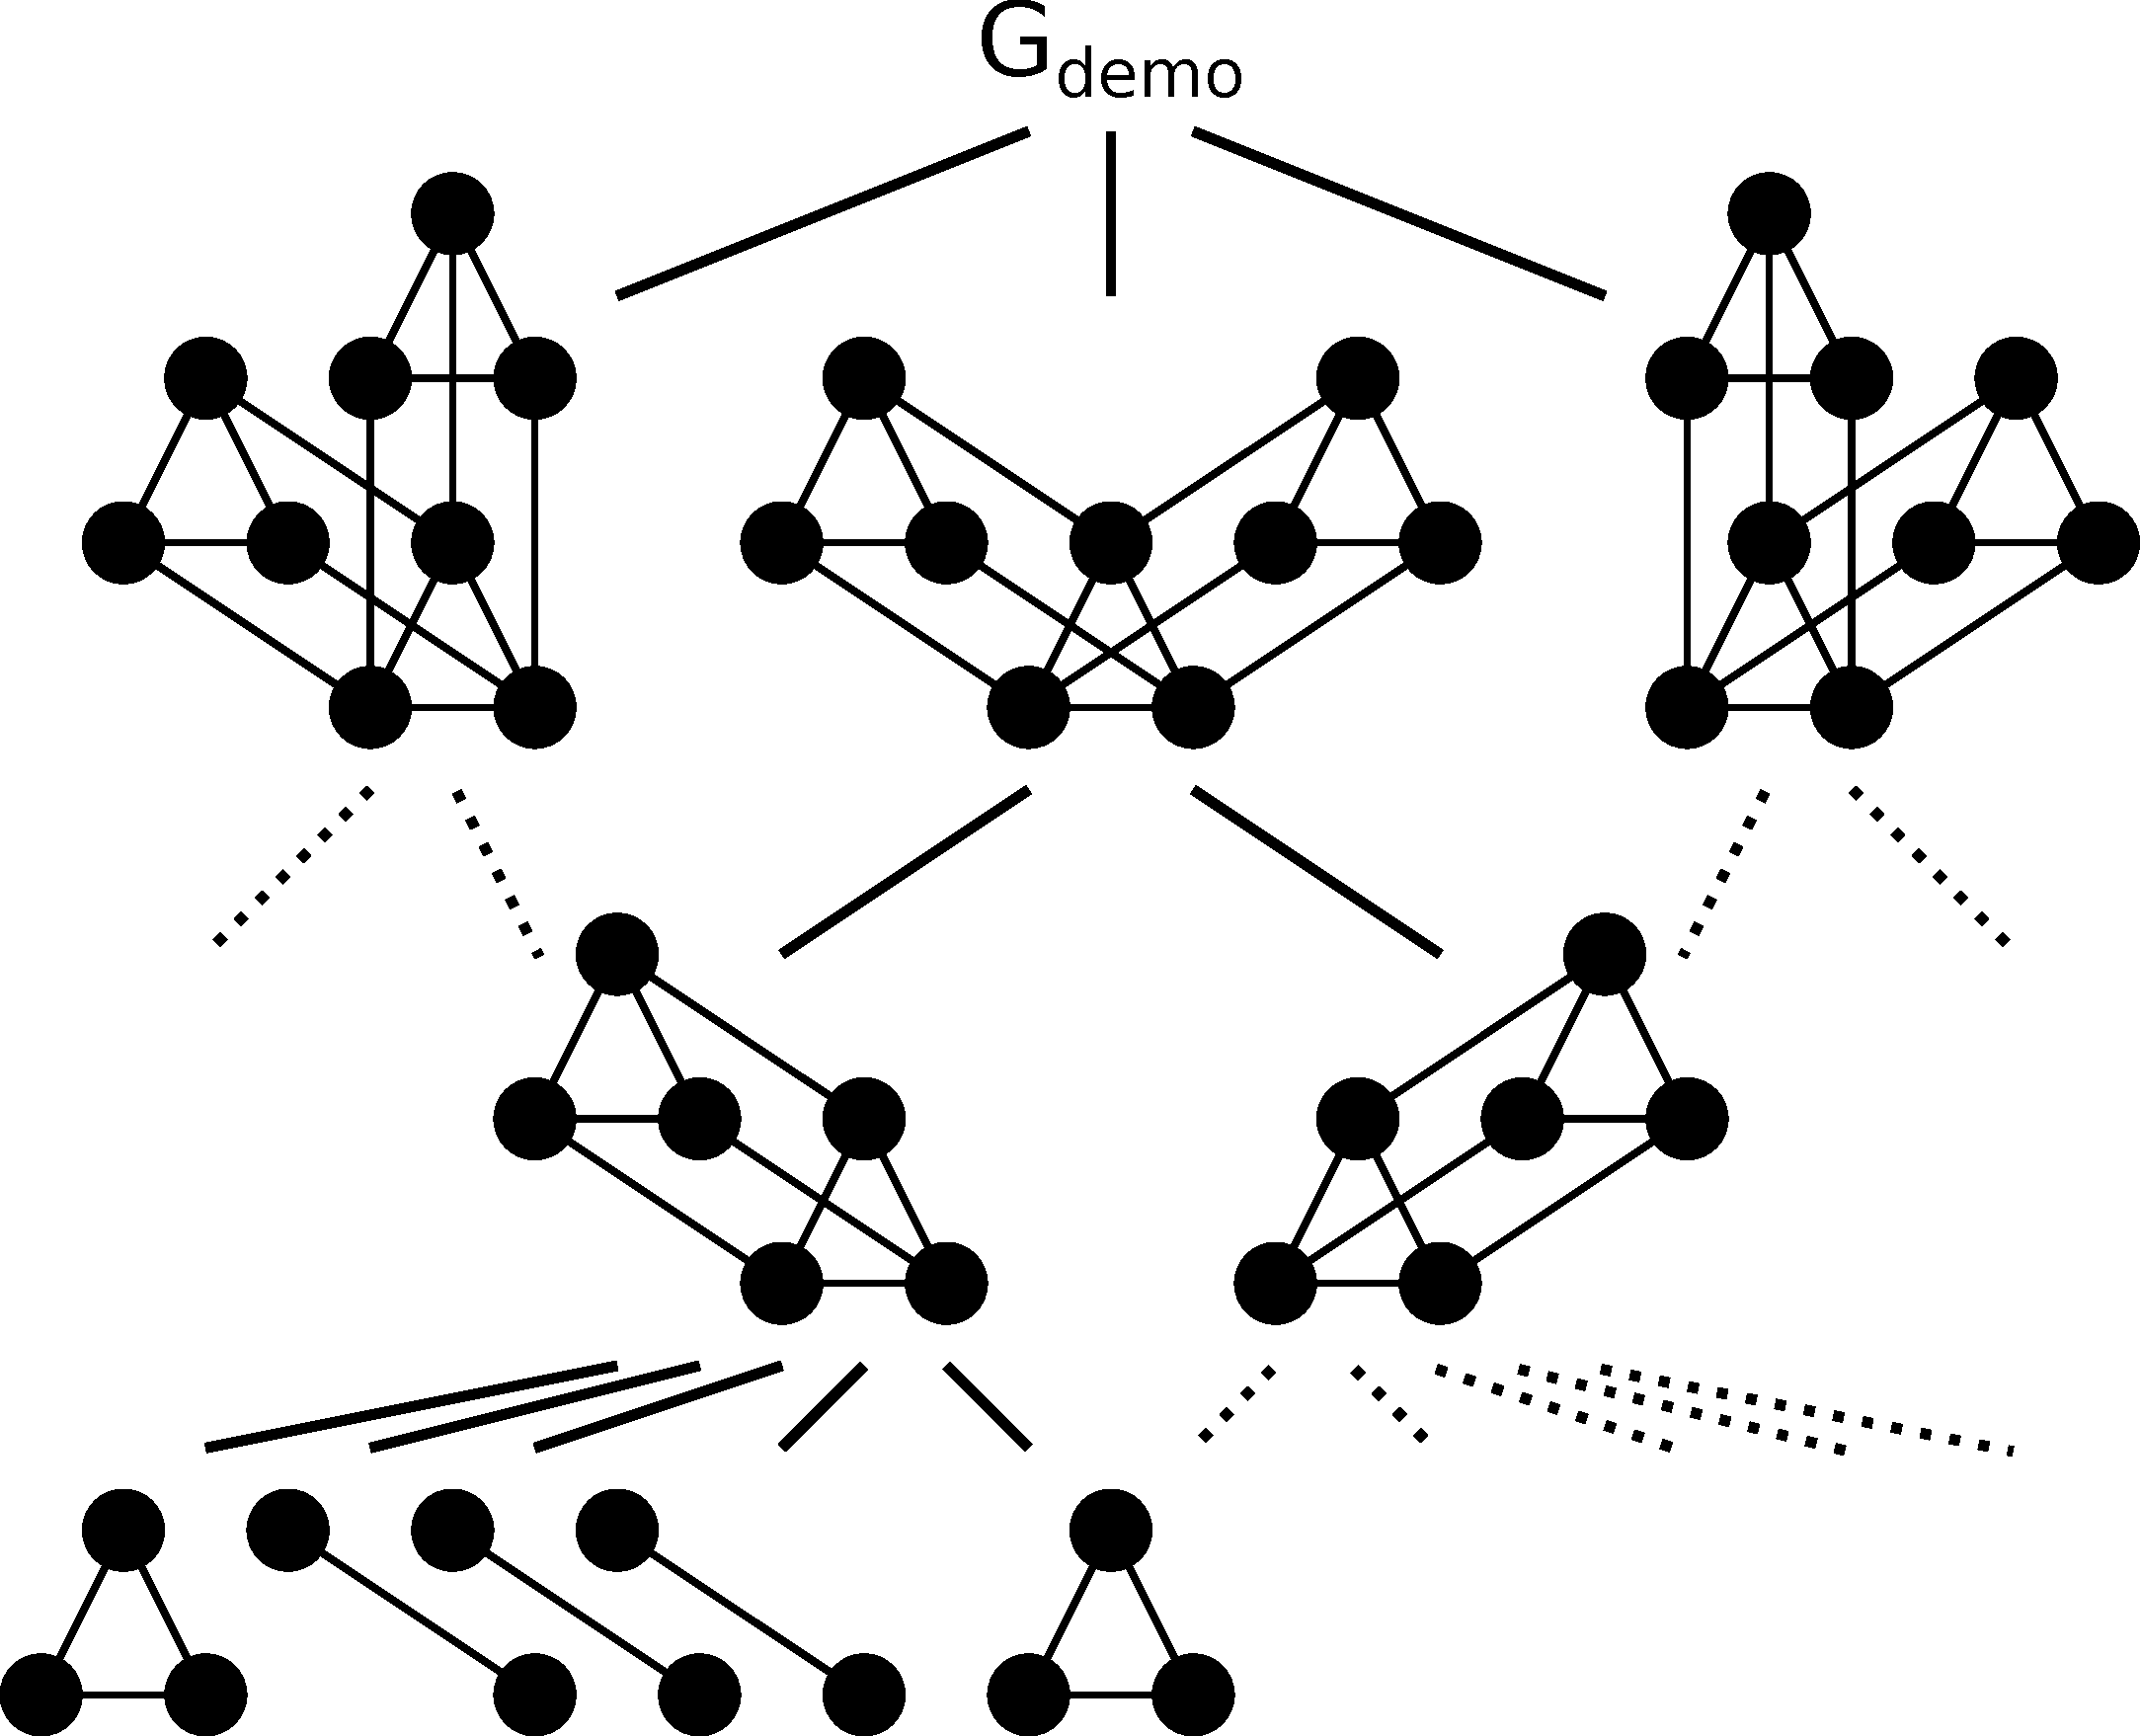
\includegraphics[width=\linewidth]{../../img/svg/3xc2c3_new_comdrp}
  %   \caption{}\label{fig:demo_graph:comdrp}
  % \end{subfigure}%
  % %
  % \hfill
  % \begin{subfigure}[t]{0.345\linewidth}\centering
  %   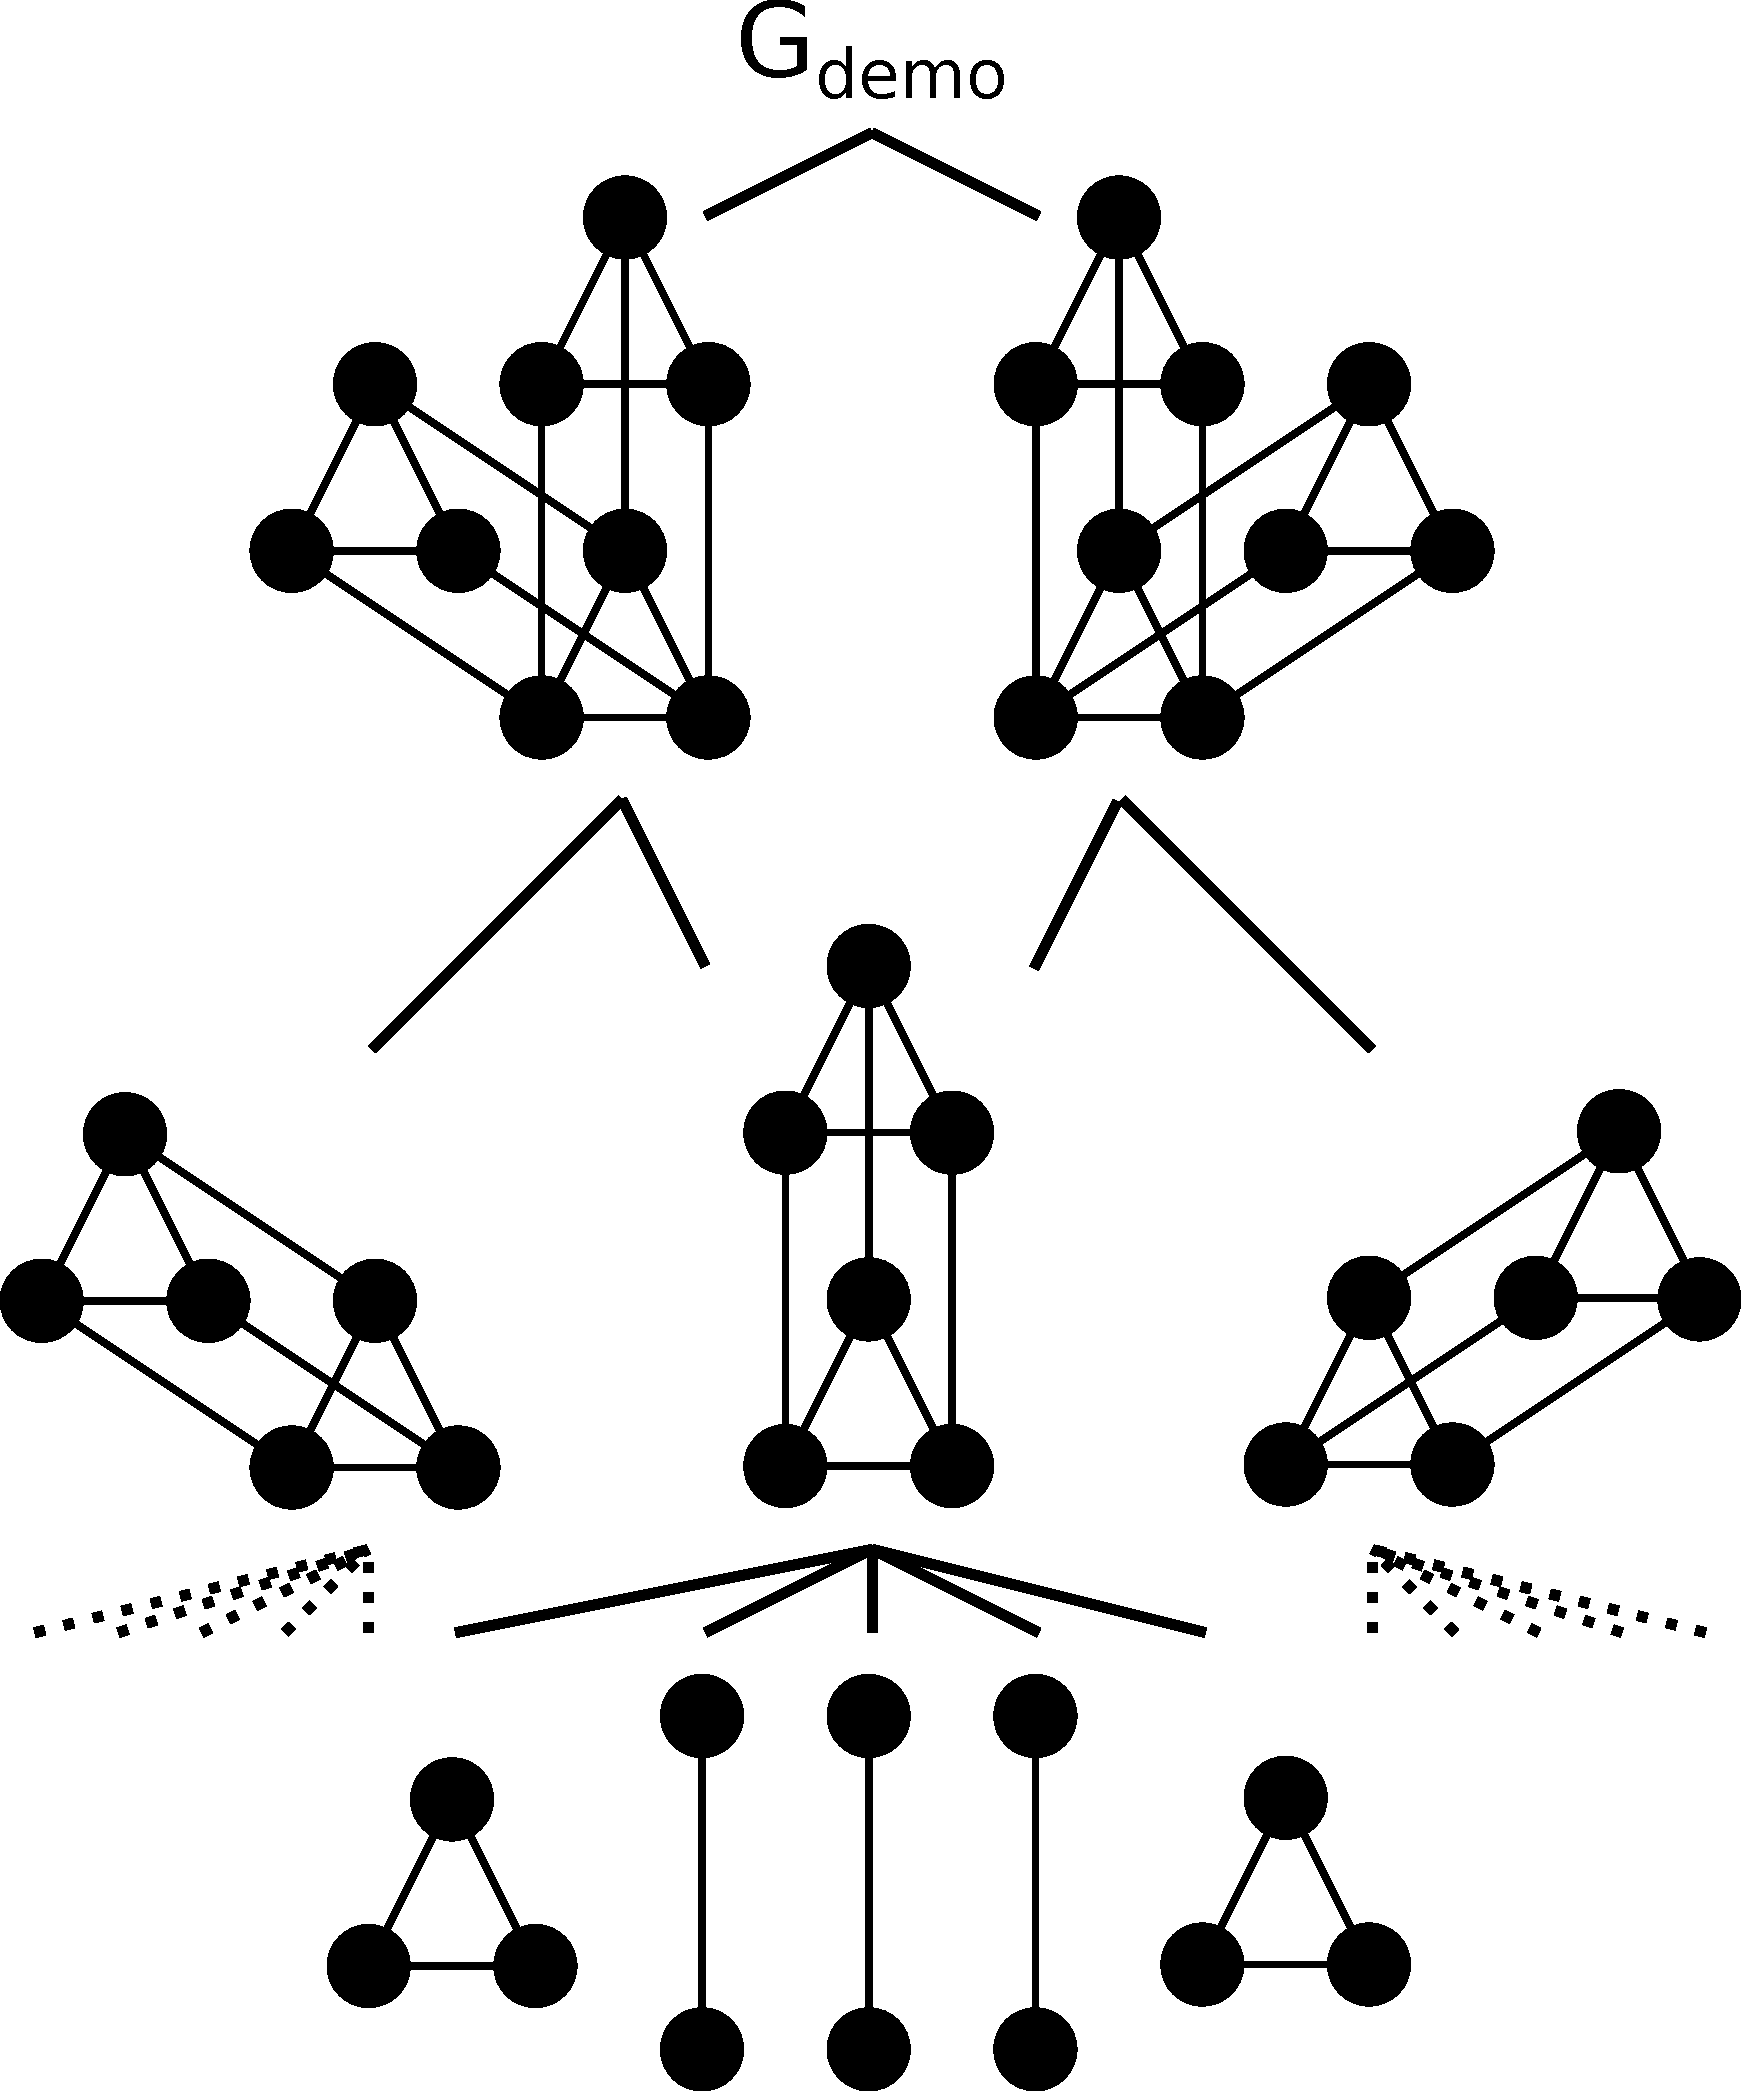
\includegraphics[width=\linewidth]{../../img/svg/3xc2c3_new_candrp}
  %   \caption{}\label{fig:demo_graph:candrp}
  % \end{subfigure}%
  %
  \caption{
  (\ref{fig:demo_graph:graph}) A graph, $G_{demo}$, used to illustrate concepts throughout this and the next section.
  %
  (\ref{fig:demo_graph:comdrp}) The complete DR-plan of $G_{demo}$.
  % i.e.\ $ComDRP(G_{demo})$.
  Dashed lines indicate that the children repeat the same pattern as the others shown on this level. The children of triangles (3 edges) are omitted.
  %
  (\ref{fig:demo_graph:candrp}) The canonical DR-plan of $G_{demo}$, which is optimal (see Section~\ref{sec:DRP}).
  % i.e.\ $OptDRP(G_{demo})$.
  The children of triangles are omitted.}
  \label{fig:demo_graph}
\end{figure*}%



% \ClearMyMinHeight
% \SetMyMinHeight{.4}{../../img/svg/triangle}
% \SetMyMinHeight{.3}{../../img/svg/triangle_candrp}
% \SetMyMinHeight{.3}{../../img/svg/triangle_clustmindrp}

%\begin{figure*}\centering%
%
%\begin{subfigure}{0.4\linewidth}\centering
%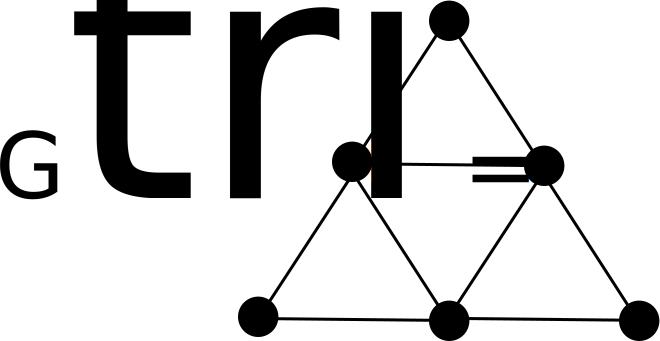
\includegraphics[height=\myMinHeight]{../../img/svg/triangle}
%    \caption{}\label{fig:demo_graph_tri:graph}
% \end{subfigure}%
%
%  \hfill
% \begin{subfigure}{0.3\linewidth}\centering
%   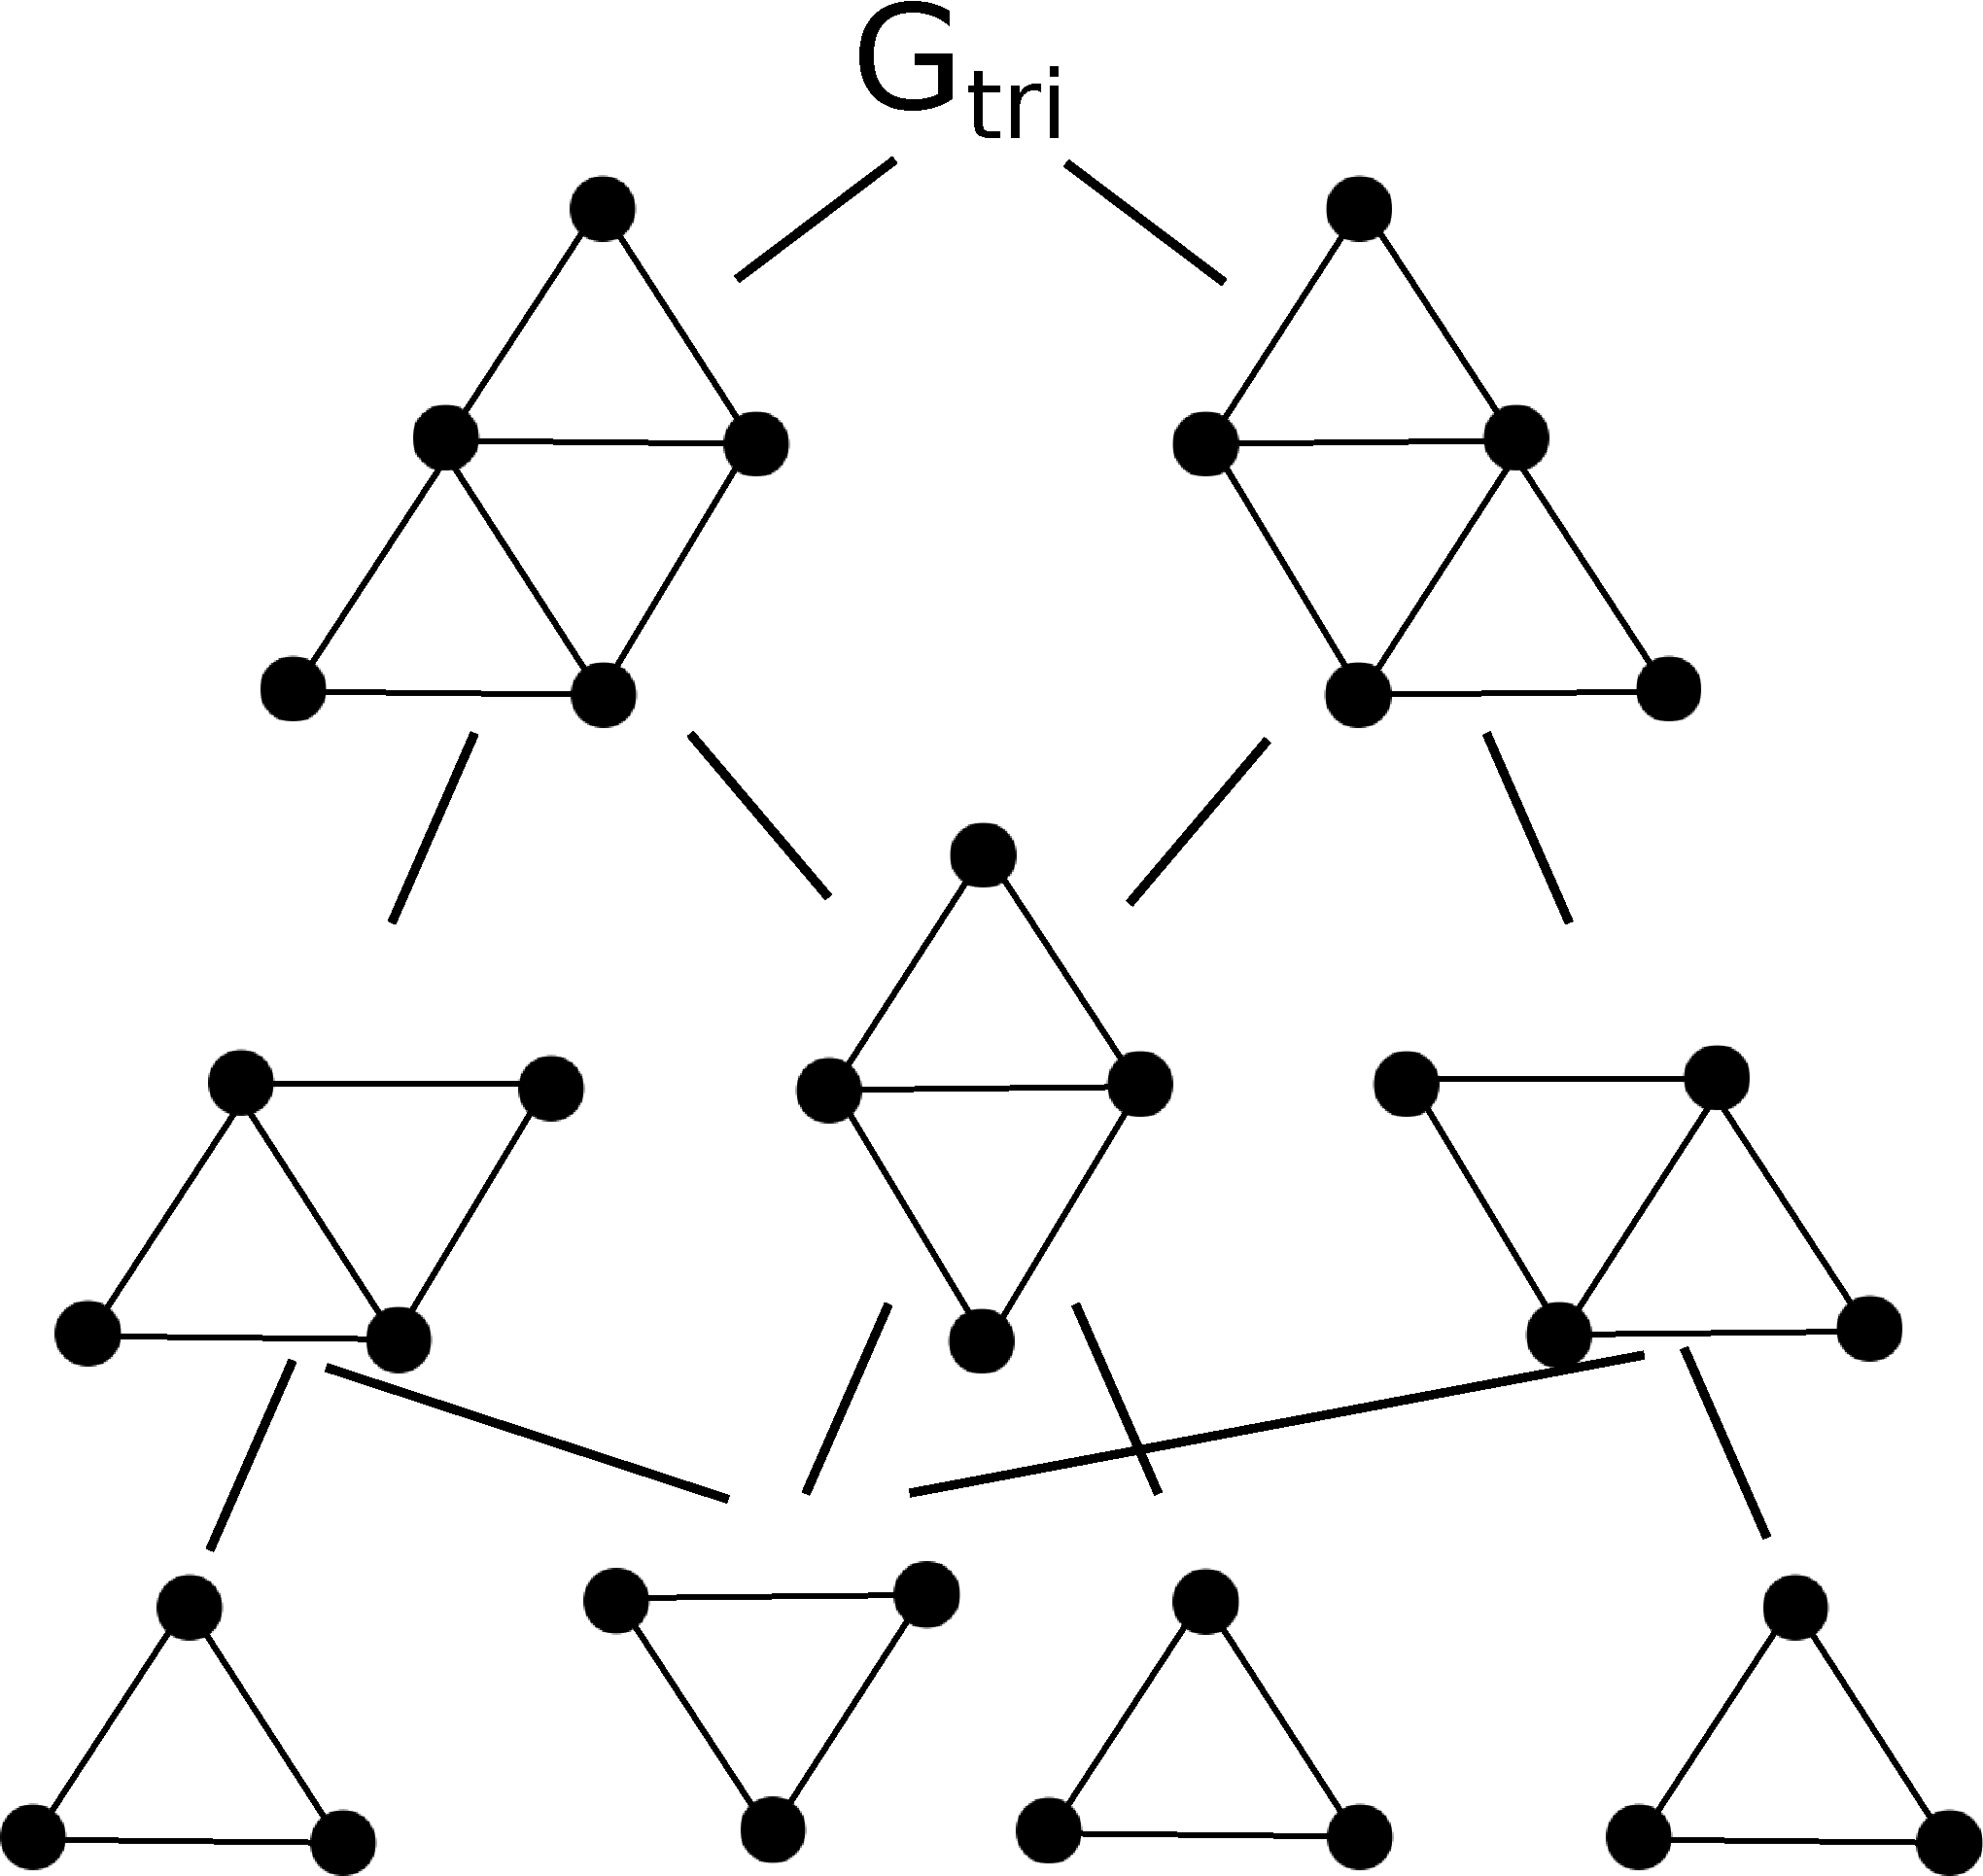
\includegraphics[height=\myMinHeight]{../../img/svg/triangle_candrp}
%    \caption{}\label{fig:demo_graph_tri:candrp}
%  \end{subfigure}%
%
%  \hfill
%  \begin{subfigure}{0.3\linewidth}\centering
%   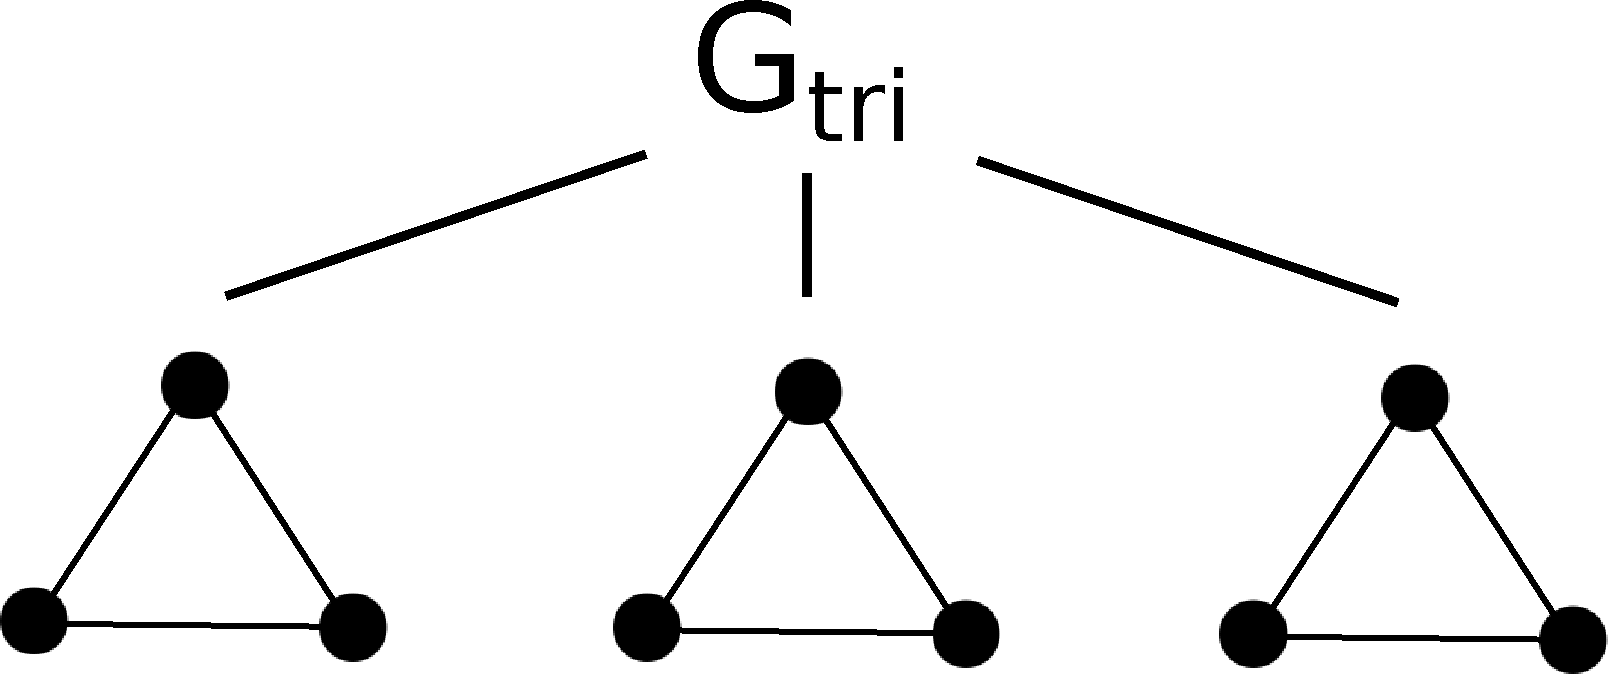
\includegraphics[height=\myMinHeight]{../../img/svg/triangle_clustmindrp}
%   \caption{}\label{fig:demo_graph_tri:clustmindrp}
%  \end{subfigure}%
%
%  \caption{(\ref{fig:demo_graph_tri:graph}) A simple graph, $G_{tri}$, of 3 triangles intersecting trivially. (\ref{fig:demo_graph_tri:candrp}) The canonical DR-plan of $G_{tri}$. (\ref{fig:demo_graph_tri:clustmindrp}) A DR-plan of graph $G_{tri}$ which gives cluster minimality  (See Section \ref{sec:prev}). Using the ideas from the paper~\cite{lomonosov2004graph}, the children of a triangle are the primitives of a point and an edge. Thus, the fan-in of this graph is 3, whereas the canonical/optimal DR-plan has fan-in of 2. With this counterexample, it is clear that cluster minimality is not sufficient for optimality.}
% \label{fig:demo_graph:clustmindrp}
%  \label{fig:demo_graph_tri}
%\end{figure*}%






% \begin{definition}\label{def:drp}
%     The \dfn{decomposition-recombination \mbox{(DR-)} plan} \cite{hoffman2001decompositionI} of graph $G$, $\drp{G}$, is defined as a forest that has the following properties:
%     \begin{enumerate}
%         \item Each node represents/contains/is a rigid subgraph of $G$.
%         % \item For a node, $C$, that is  a non-trivial graph, its $N$
%         % children, $C_1, \ldots, C_N$, are rigid vertex-maximal proper
%         % subgraphs of $C$.
%         \item The children $C_1,\ldots,C_N$ of a node $C$ satisfy $\bigcup_{i=1}^N{C_i}=C$.
%         \item A leaf node is a single edge. A \dfn{trivial} graph is empty or a single vertex. Note that a trivial graph is not isostatic.
%         \item A root node is a vertex-maximal rigid subgraph of $G$.
%     \end{enumerate}
% %
%     % It can also be described recursively as: the root is $G$, its children are the trivial subgraphs and the DR-plans of its wellconstrained vertex-maximal proper subgraphs whose union is $G$ itself.
% %
%     A DR-plan is \dfn{complete} if it satisfies an additional property: for an internal node $C$, its children are all of the rigid vertex-maximal proper subgraphs of $C$. This makes Property 2 implicit.
%   %and in fact, $C$ contains all the edges in the union of its children as well.
%   We denote a complete DR-plan of $G$ as $\comdrp{G}$.

%   A DR-plan is \dfn{optimal} if it minimizes the maximum fan-in over all nodes in the forest. The maximum  fan-in is called the \dfn{size} of the DR-plan. We denote an optimal DR-plan of $G$ as $\optdrp{G}$.
% %
% %In general, $C$ is the graph in an arbitrary node in $CompleteDRP(G)$.
% %$C_i$ is the $i^{\text{th}}$ child of $C$. It is implied that $C_i$ is
% %an isostatic vertex-maximal proper subgraph.
%     %Note that nodes will be referred to interchangeably as ``the node that
%     %represents or contains the (sub)graph $C$'' and as simply ``$C$''.
% \end{definition}



\begin{definition}
[DR-plan]
\label{def:drp}
    A \dfn{decomposition-recombination \mbox{(DR-)} plan}~\cite{hoffman2001decompositionI} of graph $G$ is defined as a forest that has the following properties:
    \begin{enumerate}
        \item Each node represents a rigid subgraph of $G$.\footnote{Nodes will be referred to interchangeably as ``the node that represents or contains the (sub)graph $C$'' and as simply ``$C$''.}
        \item A root node is a vertex-maximal rigid subgraph of $G$.
        \item A node is the subgraph of $G$ induced by the union of its children.
        \item A leaf node is a single edge.
    \end{enumerate}
\end{definition}

Note that this definition permits the same rigid subgraph to appear in multiple nodes of the DR-plan. Not permitting such duplication would, in general, require the DR-plan to be defined as a directed acyclic graph instead of a forest.

\begin{definition}
[Complete DR-plan]
    A DR-plan is \dfn{complete} if it satisfies an additional property: for an internal node $C$, its children are all of the rigid vertex-maximal proper subgraphs of $C$ (which makes Property 3 of a DR-plan implicit).
\end{definition}

\begin{definition}
[Optimal DR-plan]
    A DR-plan is \dfn{optimal} if it minimizes the maximum fan-in over all nodes in the forest.
    % The maximum fan-in is called the \dfn{size} of the DR-plan.
\end{definition}

% We denote these different kinds of DR-plans as $\drp{G}$, $\comdrp{G}$, and $\optdrp{G}$, respectively.





%
% \todo{This was labeled as both begin(remark) and end(observation), what was your intent?}
\begin{remark}
  More than one node (leaf) in a DR-plan forest may represent the same subgraph (vertex) of $G$.
  For a given graph, there could be exponentially many DR-plans---and even optimal DR-plans---in the size of the graph. A complete DR-plan is unique but may not be (and is usually not) optimal. DR-plans of self-similar graphs are self-similar.
\end{remark}

See Figures \ref{fig:demo_graph}, \ref{fig:c2c3ofk33s}, \ref{fig:demo_graph:candrpseq}, \todo{we lost this figure, replaced with \ref{fig:seqdrp_nonuniqueness}, should it be cited here now or should the other be added back in somewhere?} \ref{fig:overconstrained}, and \ref{fig:bodypindrp} for examples of DR-plans and how their properties relate to each other.


\subsection{Previous Work on DR-Plans}
\label{sec:prev}
% \todo{We now briefly survey existing techniques for studying 2D qusecs,  many of which are \dfn{bar-joint} systems (Examples 1 and 2 above, see Sections \ref{sec:prelim}, \ref{sec:DRP}, and \ref{sec:recomb}), \dfn{body-hyperpin} systems (Example 4 and 5, see Section \ref{sec:bodypin}) or \dfn{pinned-line incidence} systems (Example 3, see Section \ref{sec:pinnedline}). The limitations of these techniques directly motivate the contributions of this paper.}
We now briefly survey existing techniques for detecting rigidity and creating DR-plans of 2D constraint systems. The limitations of these techniques directly motivate the contributions of the next  section.

\subsubsection{Finding (Vertex)-Maximal, Generically Rigid Subsystems}
Fast, graph-based algorithms exist (pebble-game~\cite{Jacobs:1997:PG,hoffmann1997solvablesubsets,jermann2006decomposition,Lee:2007:PGA}), for locating all maximal, \dfn{generically rigid} subsystems \seedefs. When the input itself is rigid, these algorithms do nothing, i.e.\ compute the identity function.

However, both for self-similar or just aperiodic 2D qusecs, it is imperative to recursively decompose rigid systems into their rigid subsystems, down to the level of geometric primitives, in order to understand or design properties at all scales, such as \seedefs\ \dfn{rigidity}, \dfn{flexes}, distribution of \dfn{external stresses}, boundary conditions for \dfn{isostaticity}, as well as behavior under constraint variations.

\subsubsection{Optimal Recursive Decomposition (DR-Planning)}
Recursive decomposition of geometric constraint systems has been formalized \cite{hoffman2001decompositionI,hoffman2001decompositionII} and well-studied \cite{lomonosov2004graph,sitharam2005combinatorial,jermann2006decomposition} as the \dfn {Decomposition-Recombination (DR-) planning} problem \seedefsprelim. For the abovementioned classes of 2D qusecs, generic rigidity is a combinatorial property and hence each level of the decomposition should, in principle, be achievable by a graph-based algorithm without involving the geometric information in the constraint system. Since many such decompositions can exist for a given constraint system, criteria defining desirable or optimal DR-plans and DR-planning algorithms were given in~\cite{hoffman2001decompositionI}.
%An \dfn{optimal DR-plan} is one that minimizes the \dfn{size} \seedefsprelim, i.e., the maximum number of child subsystems of any parent system. Being exponential in the size, the complexity of solving the parent constraint system is overwhelmingly dominated by the complexity of solving the child systems.

However, for overconstrained 2D qusecs, even when restricted to bar-joint systems, the optimal DR-planning problem was shown to be NP-hard \cite{lomonosov2004graph, sitharam2005combinatorial}.
The NP-hardness of the optimal DR-planning problem for 2D bar-joint graphs is partly the consequence of possibly exponential number of DR-plans. On the other hand, although the complete DR-plan is unique it could have large average fan-in and exponentially many nodes making it far from optimal.

\subsubsection{DR-plans for Special Classes and with Other Criteria}
For a special class of 2D qusecs, namely \dfn{tree-decomposable} systems~\cite{owen1991algebraic,fudos1997graph,joan-arinyo2004revisiting} common in computer aided mechanical design (which includes ruler-and-compass and Henneberg-I constructible systems), all DR-plans turn out to be optimal. This satisfies the Church-Rosser property, leading to highly efficient DR-planning algorithms. For general 2D qusecs, alternate criteria were suggested such as \dfn{cluster minimality} requiring parent systems to have a minimal set of at least 2 rigid proper subsystems as children (i.e.\ the union of no proper subset of size at least 2 child subsystems forms a rigid system); and \dfn{proper maximality}, requiring child subsystems to be maximal rigid proper subsystems of the parent system. \seedefsc.

While polynomial time algorithms were given to generate DR-plans meeting the cluster minimality criterion~\cite{lomonosov2004graph}, no such algorithm is known for the latter criterion.
%Moreover, cluster minimality does not imply optimality as shown in Figure \ref{fig:demo_graph_tri}

% \begin{definition}
%     The \textbf{complete DR-plan} of graph $G$, $CompleteDRP(G)$, is the unique DR-plan but with a modified rule number 2: the children are \emph{all} of the trivial or wellconstrained vertex-maximal proper subgraphs of that node $C$. By this, rule 3 is implicit for a complete DR-plan.
% \end{definition}

% \begin{definition}
%     The \textbf{optimal DR-plan} of graph $G$, $OptimalDRP(G)$, is the DR-plan that minimizes the maximum fan-in over all nodes in the forest. It is not necessarily unique.
% \end{definition}




%\emph{wellconstrained} bar and joint graph with values $(V,E,w_V,w_E)$.
% \todo{I don't think the following is actually necessary to mention...} To keep problems meaningful we assume that $G$ is connected, as the methods discussed are used to solve systems of equations to establish linkages. It is not useful to solve for two bodies simultaneously if there are no constraints between them.
% THIS MEANS NO EDGES MAY BE LEFT OUT, ALSO.




%\subsection{DR-plan}
%%\subsection{Definitions}
%%\label{sec:prelim_defs}
%%
%%% TODO
%%
%%% A paragraph of preliminaries such as:
%%%     - rigidity matrix R,
%%%     - stress vectors S one coordinate per edge (w/ SR =E (external stress vector, 2 coordinates  per vertex));
%%%     - flex vectors F (2 coordinates per vertex) (right nullspace/kernel of R)
%%% Should precede the definition of
%%%     + independent,
%%%     + overconstrained (not independent),
%%%     - rigid (contains an independent set with sufficiently many eedges/constraints)
%%%     - isostatic (wellconstrained/minimally rigid), ,
%%%     - flexible (not rigid),
%%%     + underconstrained (independent and not rigid).
%%% After that, define DR plans etc.
%%
%%In Sections \ref{sec:DRP} and \ref{sec:recomb} a \textbf{graph} is a bar and joint system. $G=(V,E,w_V,w_E)$ is a set of vertices, $V$, and a set of edges, $E$, defined as a tuple of vertices from $V$ (undirected). Additionally, there are two weight functions, $w_V: V \to \mathbb{R}^+$ and $w_E: E \to \mathbb{R}^+$. The \textbf{density} of graph $G$ is $d(G) = \sum_{e\in E}{w_E(e)} - \sum_{v\in V}{w_V(v)}$.
%%
%%Given a constant $k$, a graph $G$ is:
%%\begin{itemize}
%%    \item \textbf{independent} (or \textbf{sparse}) if, for all non-trivial subgraphs $S\subseteq G$, $d(S) \leq k$.
%%
%%    \item \textbf{overconstrained} if it is not independent.
%%
%%    \item \textbf{wellconstrained} (or \textbf{tight}) if $G$ is independent and $d(G)=k$.
%%
%%    \item \textbf{rigid} if there exists some spanning subgraph $S\subseteq G$ such that $S$ is wellconstrained.
%%
%%    \item \textbf{underconstrained} if $G$ is independent and not rigid.
%%
%%    % \item \textbf{trivial} if (1) it is overconstrained graph and (2) all of its subgraphs are also trivial. Trivial graphs are input.
%%\end{itemize}
%%
%\textbf{Trivial} graphs are ill-defined in the general case. The only strict requirements are: (1) it must overconstrained and (2) all of its subgraphs are also trivial.
%
%% \begin{definition}
%%     A graph is \textbf{overconstrained} if, given constant $k$, there exists some
%%     % induced
%%     subgraph $S\subseteq G$ such that $d(S) > k$.
%% \end{definition}
%
%% \begin{definition}
%%     A graph is \textbf{wellconstrained} if, given constant $k$, $d(G) = k$ and for all
%%     % induced
%%     subgraphs $S\subseteq G$, (1) $d(S)\leq k$, or (2) given a set of trivial graphs $T$, $S$ is isomorphic to one of the graphs in $T$ (i.e.\ $S$ is trivial).
%% \end{definition}
%
%
%
%% \begin{definition}
%%     A \textbf{trivial} graph is ill-defined in the general case. The only strict requirements are: (1) it must be an overconstrained graph and (2) all of its subgraphs are also trivial.
%%     \todo{Maybe leave the following out until it's needed later?}
%%     In the familiar geometric cases of $d$-dimensional space, all vertex weights are $d$, all edge weights are $1$, and constant $k= -{{d+1}\choose{2}}$. Trivial graphs for 2D would be a single vertex. Trivial graphs in 3D would be a vertex and an edge (2 vertices with an edge between). Etc. These trivial graphs capture the notion of the rotational symmetry that exists in geometric spaces.
%% \end{definition}
%
%
%\begin{definition}\label{def:drp}
%    The \textbf{decomposition-recombination \mbox{(DR-)} plan} of graph $G$, $DRP(G)$, is defined as a tree that has the following properties:
%    \begin{enumerate}
%        \item The root of the tree `contains' $G$.
%        \item For all nodes, $C$, that `contain' non-trivial graphs, its $N$ children, $C_1, \ldots, C_N$, are trivial or wellconstrained vertex-maximal proper subgraphs of that node $C$.
%        \item The vertex set of $\bigcup_{i=1}^N{C_i}$ is the vertex set of $C$.
%        \item A node with a trivial subgraph is a leaf.
%    \end{enumerate}
%
%    % It can also be described recursively as: the root is $G$, its children are the trivial subgraphs and the DR-plans of its wellconstrained vertex-maximal proper subgraphs whose union is $G$ itself.
%
%    An equivalent DAG can be constructed from this tree such that all nodes containing the same subgraphs are combined into one, with all edges preserved.
%
%    Note that nodes will be referred to interchangeably as ``the node that contains the (sub)graph $C$'' and as simply ``$C$''.
%
%    A DR-plan is \textbf{complete} if it satisfies the modified rule number 2: the children are \emph{all} of the trivial or wellconstrained vertex-maximal proper subgraphs of that node $C$. This makes rule 3 implicit. The complete DR-plan is unique.
%
%    A DR-plan is \textbf{optimal} if it minimizes the maximum fan-in over all nodes in the forest. It is not necessarily unique.
%\end{definition}
%
%% \begin{definition}
%%     The \textbf{complete DR-plan} of graph $G$, $CompleteDRP(G)$, is the unique DR-plan but with a modified rule number 2: the children are \emph{all} of the trivial or wellconstrained vertex-maximal proper subgraphs of that node $C$. By this, rule 3 is implicit for a complete DR-plan.
%% \end{definition}
%
%% \begin{definition}
%%     The \textbf{optimal DR-plan} of graph $G$, $OptimalDRP(G)$, is the DR-plan that minimizes the maximum fan-in over all nodes in the forest. It is not necessarily unique.
%% \end{definition}
%
%
%\subsection{Notation}
%
%In Sections \ref{sec:DRP} and \ref{sec:recomb}, $G$ is taken to be a \emph{wellconstrained} bar and joint graph with values $(V,E,w_V,w_E)$.
%% \todo{I don't think the following is actually necessary to mention...} To keep problems meaningful we assume that $G$ is connected, as the methods discussed are used to solve systems of equations to establish linkages. It is not useful to solve for two bodies simultaneously if there are no constraints between them.
%% THIS MEANS NO EDGES MAY BE LEFT OUT, ALSO.
%
%$Idc(G,X)$ is the graph induced on $G$ with the vertex set $X\subseteq V$. This can also be overloaded such that, using graph $H=(W,F)$, $Idc(G,H)=Idc(G,W)$.
%
%$C$ is the graph in an arbitrary node in $CompleteDRP(G)$. $C_i$ is the $i^{\text{th}}$ child of $C$. By definition of a DR-plan, it is implied that $C_i$ is a wellconstrained vertex-maximal proper subgraph.


\section{The canonical DR-plan}
\label{sec:DRP}
% In the problem of the optimal DR-Plan there is generally not a unique plan.
% % Indeed, we will prove a union of $N$ isostatic subgraphs will result in $N$ unique plans, but that at the $N^{\text{th}}$ level of the tree it will always be the same. Therefore, all choices of decomposition are in some sense equivalent. The theorem we seek to prove is thus:
% However, we will show that regardless of which children are chosen for the plan, so long as they satisfy the definition of an optimal DR-plan, the recombination will require solving of the same systems. Being the smallest such structure that offers this, the definition of an optimal DR-plan could be considered the canonical DR-plan.
% % To assist in showing this, we prove this core theorem throughout this section:

% In this section, we discuss 2D bar-joint graphs. All vertex weights are $2$, all edge weights are $1$, and constant $k= -{{3}\choose{2}}=-3$. Trivial graphs are a single vertex and empty set. Furthermore, 2D isostatic graphs must be connected.
% % The greatest density of a 2D isostatic graph is $-2$ (the vertex). The other disconnected part of the graph would need to have a density of $-1$, which is overconstrained and not possible in a isostatic graph (because there is no trivial graph with that density).

The NP-hardness of the DR-planning problem for 2D bar-joint graphs is partly the consequence of possibly exponential number of DR-plans. On the other hand, although the complete DR-plan is unique it could have large average fan-in and exponentially many nodes making it far from optimal.

In this section we define a \dfn{canonical} plan to capture those aspects of an optimal DR-plan that mimic a complete DR-plan's uniqueness, while for independent (underconstrained or isostatic graphs), we show that the nonunique parts do not affect optimality.

\begin{definition}\label{def:canonical_drplan}
    The \dfn{canonical DR-plan} satisfies the following three properties:
    (1) it is a DR-plan;
    (2) children are rigid vertex-maximal proper subgraphs of the parent; and
    (3) if all pairs of rigid vertex-maximal proper subgraphs intersect trivially then all of them are children, otherwise take as children exactly two that intersect non-trivially.
\end{definition}

This definition gives the canonical DR-plan a surprisingly strong Church-Rosser property.

\begin{theorem}
\label{theorem:canonical_exists_and_is_optimal}
\label{theorem:canonical_is_optimal}
\label{theorem:main}
    A canonical DR-plan exists and any canonical DR-plan is optimal.
\end{theorem}


% \begin{theorem} \label{theorem:canonical_is_optimal}
%     \label{theorem:main}
%     Any canonical DR-plan is an optimal DR-plan.
% \end{theorem}

%The proof of this theorem is a direct consequence of the following  more general theorem.

%\begin{theorem}\label{theorem:main}
%Given an isostatic 2D bar-joint graph $G$ and ComDRP$(G)$, for all nodes $C$
%with children $C_1,\ldots,C_N$ preserve children according to the following rules.
%\begin{enumerate}
%    \item If $C_i \cap C_j$ is trivial then keep all $C_1,\ldots,C_N$ as children.
%    \item If $C_i \cap C_j$ is isostatic then select any two out of $C_1,\ldots,C_N$ as children.
%\end{enumerate}
%This is a canonical DR-plan.
%\end{theorem}


This theorem (proven in the \ref{theorem:main:proof}) relies on the following crucial observation and lemma that are also used for other types of qusecs in the Application sections (\ref{sec:bodypin}, \ref{sec:pinnedline}) of the paper.

\begin{observation}\label{lemma:union_intersection}
If $F_i$ and $F_j$ are isostatic subgraphs of the same
isostatic graph $F$, \
then the following hold:
(1) $F_i\cup F_j$ is not trivial;
(2) $F_i\cup F_j$ is underconstrained if and only if $F_i\cap F_j$ is trivial;
(3) $F_i\cup F_j$ is isostatic if and only if $F_i\cap F_j$ is isostatic; and
(4) $F_i\cap F_j$ is not underconstrained.
\end{observation}

Then the following key properties hold at the nodes of a canonical DR-plan.

\begin{lemma}\label{lemma:combined_lemma}
Let $C$ be a node of a canonical DR-plan, with distinct children $C_i$ and $C_j$
Then
\begin{enumerate}
    \item\label{lemma:wc_intersection_is_C}
    $C_i\cup C_j$ is isostatic if and only if $C_i\cup C_j = C$.

    \item\label{lemma:wc_intersection_makes_all_wc}
    If $C_i\cup C_j$ is isostatic, then $\forall k: C_i\cup C_k$ is isostatic. Alternatively, if $C_i\cup C_j=C$, then $\forall k: C_i\cup C_k=C$.

    \item\label{lemma:uc_intersection_makes_all_uc}
    If $C_i\cap C_j$ is trivial, then $\forall k: C_i\cap C_k$ is trivial.
\end{enumerate}
\end{lemma}

\begin{remark}
The first item in the above lemma generalizes to the union of any number of children, $C_1,\ldots,C_k$, resulting in the desirable property of \dfn{Cluster Minimality}, defined in \cite{hoffman2001decompositionI} holding for these canonical-optimal DR-plans.
\end{remark}






% \begin{figure*}\centering
% \begin{subfigure}{.3\linewidth}\centering
%     % \newcommand{\tedge}[5]{\draw[#3] (#1)-- node[e, #5] (e#4) {#4} (#2)}

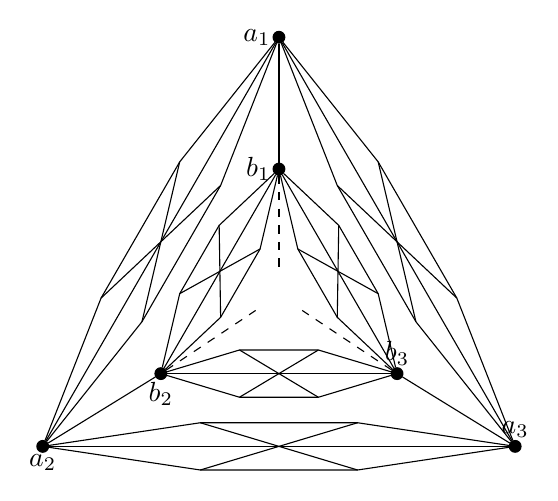
\begin{tikzpicture}[scale=3]
    \tikzstyle{v}=[draw, circle, minimum size=0.75cm]
    \tikzstyle{c}=[draw, circle, inner sep=1.5, fill=black]
    \tikzstyle{e}=[]

    \node[circle,fill=white,inner sep=7] (center) at (0,0-.125-.1) {};

    \node[c] (v1) at (0,0.866) [label={left,inner sep=.555}:$a_1$]{};
    \node[c] (v2) at (-1,-0.866) [label={below,inner sep=.555}:$a_2$]{};
    \node[c] (v3) at (1,-0.866) [label={above,inner sep=.555}:$a_3$]{};

    \node[c] (v4) at (0,0.433-.125) [label={left,inner sep=.555}:$b_1$]{};
    \node[c] (v5) at (-0.5,-0.433-.125) [label={below,inner sep=.555}:$b_2$]{};
    \node[c] (v6) at (0.5,-0.433-.125) [label={above,inner sep=.555}:$b_3$]{};

    \tedge{v1}{v2}{solid}{}{};
    \tedge{v1}{v3}{solid}{}{};
    \tedge{v2}{v3}{solid}{}{};

    \tedge{v4}{v5}{solid}{}{};
    \tedge{v4}{v6}{solid}{}{};
    \tedge{v5}{v6}{solid}{}{};


    \tedge{v1}{v4}{solid}{}{};
    \tedge{v2}{v5}{solid}{}{};
    \tedge{v3}{v6}{solid}{}{};


    \tedge{v4}{center}{dashed}{}{};
    \tedge{v5}{center}{dashed}{}{};
    \tedge{v6}{center}{dashed}{}{};


    % sin(30deg) = 0.5
    % cos(30deg) = 0.866

    % o/i -> outside/inside triangle
    % b/l/r -> bottom/left/right edge of triangle

    \coordinate (ob0) at (-0.333,-0.866-0.1);
    \coordinate (ob1) at (0.333,-0.866-0.1);
    \coordinate (ob2) at (-0.333,-0.866+0.1);
    \coordinate (ob3) at (0.333,-0.866+0.1);
    \draw (v2) -- (ob0) -- (ob1) -- (v3);
    \draw (v2) -- (ob2) -- (ob3) -- (v3);
    \draw (ob0) -- (ob3);
    \draw (ob2) -- (ob1);

    \draw[rotate around={60:(-1,-0.866)}] (v2) -- (-0.333,-0.766) -- (0.333,-0.766) -- (v1);
    \draw[rotate around={60:(-1,-0.866)}]  (v2) -- (-0.333,-0.966) -- (0.333,-0.966) -- (v1);
    \draw[rotate around={60:(-1,-0.866)}]  (-0.333,-0.766) -- (0.333,-0.966);
    \draw[rotate around={60:(-1,-0.866)}]  (-0.333,-0.966) -- (0.333,-0.766);

    \draw[rotate around={-60:(1,-0.866)}] (v3) -- (0.333,-0.766) -- (-0.333,-0.766) -- (v1);
    \draw[rotate around={-60:(1,-0.866)}]  (v3) -- (0.333,-0.966) -- (-0.333,-0.966) -- (v1);
    \draw[rotate around={-60:(1,-0.866)}]  (-0.333,-0.766) -- (0.333,-0.966);
    \draw[rotate around={-60:(1,-0.866)}]  (-0.333,-0.966) -- (0.333,-0.766);




    \coordinate (ib0) at (-0.167,-0.433-.125-0.1); %(-.167,-.658)
    \coordinate (ib1) at (0.167,-0.433-.125-0.1); %(.167,-.658)
    \coordinate (ib2) at (-0.167,-0.433-.125+0.1);%(-.167,-.458)
    \coordinate (ib3) at (0.167,-0.433-.125+0.1);%(.167,-.458)
    \draw (v5) -- (ib0) -- (ib1) -- (v6);
    \draw (v5) -- (ib2) -- (ib3) -- (v6);
    \draw (ib0) -- (ib3);
    \draw (ib2) -- (ib1);

    \draw[rotate around={60:(-0.5,-0.558)}] (v5) -- (-.167,-.658) -- (.167,-.658) -- (v4);
    \draw[rotate around={60:(-0.5,-0.558)}]  (v5) -- (-.167,-.458) -- (.167,-.458) -- (v4);
    \draw[rotate around={60:(-0.5,-0.558)}]  (-.167,-.658) -- (.167,-.458);
    \draw[rotate around={60:(-0.5,-0.558)}]  (-.167,-.458) -- (.167,-.658);

    \draw[rotate around={-60:(0.5,-0.558)}] (v6) -- (.167,-.658) -- (-.167,-.658) -- (v4);
    \draw[rotate around={-60:(0.5,-0.558)}]  (v6) -- (.167,-.458) -- (-.167,-.458) -- (v4);
    \draw[rotate around={-60:(0.5,-0.558)}]  (-.167,-.658) -- (.167,-.458);
    \draw[rotate around={-60:(0.5,-0.558)}]  (-.167,-.458) -- (.167,-.658);
% \newcommand{\tedge}[5]{\draw[#3] (#1)-- node[e, #5] (e#4) {#4} (#2)}

    % \draw (-1,-0.866) -- (-0.333,-0.966);

\end{tikzpicture}

%     \caption{}\label{fig:c2c3ofk33s:a}
% \end{subfigure}%
% \begin{subfigure}{.7\linewidth}\centering
%     % \newcommand{\tedge}[5]{\draw[#3] (#1)-- node[e, #5] (e#4) {#4} (#2)}

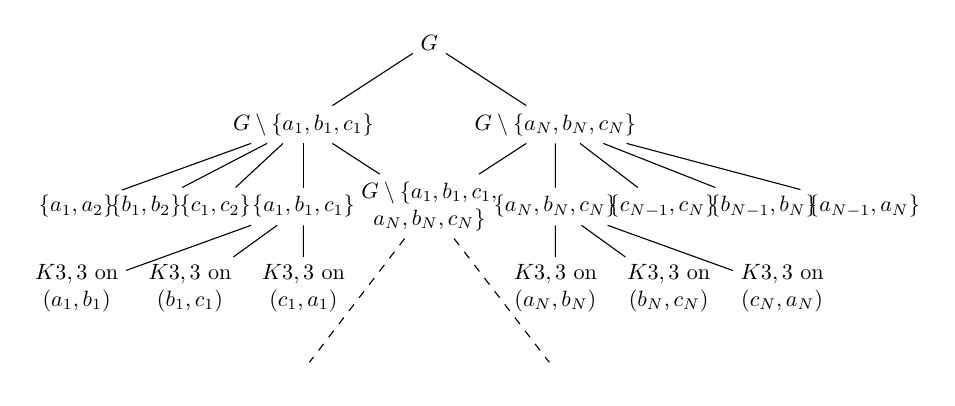
\begin{tikzpicture}[scale=.8, transform shape]
    \tikzstyle{v}=[draw, circle, minimum size=0.75cm, font=\footnotesize]
    % \tikzstyle{b}=[draw, font=\footnotesize]
    \tikzstyle{b}=[align=center]
    \tikzstyle{e}=[]

    \node[b] (c0) at (0,0*1.3) {$G$};
    \node[b] (c1a) at (-2,-1*1.3) {$G\setminus\{a_1,b_1,c_1\}$};
    \node[b] (c1b) at (2,-1*1.3) {$G\setminus\{a_N,b_N,c_N\}$};
    \node[b] (c2b) at (0,-2*1.3) {$G\setminus\{a_1,b_1,c_1,$ \\ $a_N,b_N,c_N\}$};
    \node[b] (c2a) at (-2,-2*1.3) {$\{a_1,b_1,c_1\}$};
    \node[b] (c2c) at (2,-2*1.3) {$\{a_N,b_N,c_N\}$};
    \node[b] (c2ab1) at (-5.6,-2*1.3) {$\{a_1,a_2\}$};
    \node[b] (c2ab2) at (-4.5,-2*1.3) {$\{b_1,b_2\}$};
    \node[b] (c2ab3) at (-3.4,-2*1.3) {$\{c_1,c_2\}$};
    \node[b] (c2bc1) at (6.9,-2*1.3) {$\{a_{N-1},a_N\}$};
    \node[b] (c2bc2) at (5.3,-2*1.3) {$\{b_{N-1},b_N\}$};
    \node[b] (c2bc3) at (3.7,-2*1.3) {$\{c_{N-1},c_N\}$};

    \node[b] (ab1k33) at (-5.6,-3*1.3) {$K3,3$ on \\ $(a_1,b_1)$};
    \node[b] (bc1k33) at (-7.6/2,-3*1.3) {$K3,3$ on \\ $(b_1,c_1)$};
    \node[b] (ca1k33) at (-2,-3*1.3) {$K3,3$ on \\ $(c_1,a_1)$};

    \node[b] (abNk33) at (2,-3*1.3) {$K3,3$ on \\ $(a_N,b_N)$};
    \node[b] (bcNk33) at (7.6/2,-3*1.3) {$K3,3$ on \\ $(b_N,c_N)$};
    \node[b] (caNk33) at (5.6,-3*1.3) {$K3,3$ on \\ $(c_N,a_N)$};


    \node[b] (c3a) at (-2,-4*1.3) {};
    \node[b] (c3b) at (2,-4*1.3) {};


    \tedge{c0}{c1a}{solid}{}{};
    \tedge{c0}{c1b}{solid}{}{};

    \tedge{c1a}{c2ab1}{solid}{}{};
    \tedge{c1a}{c2ab2}{solid}{}{};
    \tedge{c1a}{c2ab3}{solid}{}{};
    \tedge{c1a}{c2a}{solid}{}{};
    \tedge{c1a}{c2b}{solid}{}{};

    \tedge{c1b}{c2bc1}{solid}{}{};
    \tedge{c1b}{c2bc2}{solid}{}{};
    \tedge{c1b}{c2bc3}{solid}{}{};
    \tedge{c1b}{c2b}{solid}{}{};
    \tedge{c1b}{c2c}{solid}{}{};

    \tedge{c2a}{ab1k33}{solid}{}{};
    \tedge{c2a}{bc1k33}{solid}{}{};
    \tedge{c2a}{ca1k33}{solid}{}{};
    \tedge{c2c}{abNk33}{solid}{}{};
    \tedge{c2c}{bcNk33}{solid}{}{};
    \tedge{c2c}{caNk33}{solid}{}{};

    \tedge{c2b}{c3a}{dashed}{}{};
    \tedge{c2b}{c3b}{dashed}{}{};
\end{tikzpicture}

%     \caption{}\label{fig:c2c3ofk33s:b}
% \end{subfigure}

% \caption{(\ref{fig:c2c3ofk33s:a}) A doublet ($C_2 \times C_3$) with each edge of the triangles replaced by a $K_{3,3}$. This pattern continues inwards for a total of $N$ triangles, indicated by the dashed lines. (\ref{fig:c2c3ofk33s:b}) Most of the DR-plan of this graph, omitting further decomposition of $K_{3,3}$ subgraphs into the separate 9 edges and of edges into the component nodes. $G\setminus\{a_i,b_i,c_i\}$ is shorthand for $G$ difference those nodes and all of the nodes in the corresponding $K_{3,3}$ subgraphs. The dashed lines indicated that this exact structure is repeated.}
% \label{fig:c2c3ofk33s}
% \end{figure*}


% \FigInit
%     {(\ref{fig:c2c3ofk33s:a}) A doublet ($C_2 \times C_3$) with each edge of the triangles replaced by a $K_{3,3}$. This pattern continues inwards for a total of $N$ triangles, indicated by the dashed lines. (\ref{fig:c2c3ofk33s:b}) Most of the DR-plan of this graph, omitting further decomposition of $K_{3,3}$ subgraphs into the separate 9 edges and of edges into the component nodes. $G\setminus\{a_i,b_i,c_i\}$ is shorthand for $G$ difference those nodes and all of the nodes in the corresponding $K_{3,3}$ subgraphs. The dashed lines indicated that this exact structure is repeated.}
%     {fig:c2c3ofk33s}
% \FigTwoSubfigWithWidth
%     {.3}
%     {img/epsfromtikz/c2c3_of_k33s-0}
%     {}
%     {fig:c2c3ofk33s:a}
%     %
%     {.7}
%     {img/epsfromtikz/c2c3_of_k33s-1}
%     {}
%     {fig:c2c3ofk33s:b}


\ClearMyMinHeight
\SetMyMinHeight{.3}{img/epsfromtikz/c2c3_of_k33s-0}
\SetMyMinHeight{.7}{img/epsfromtikz/c2c3_of_k33s-1}

\begin{figure*}\centering%
    %
    \begin{subfigure}{0.3\linewidth}\centering
        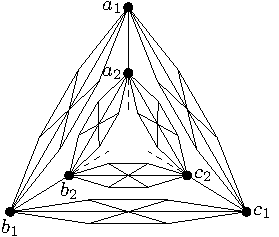
\includegraphics[height=\myMinHeight]{img/epsfromtikz/c2c3_of_k33s-0}
        \caption{}\label{fig:c2c3ofk33s:a}
    \end{subfigure}%
    %
    \hfill
    \begin{subfigure}{0.7\linewidth}\centering
        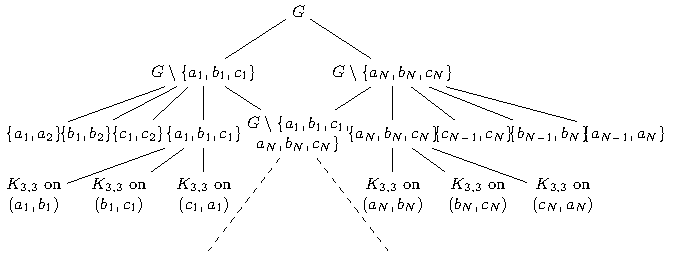
\includegraphics[height=\myMinHeight]{img/epsfromtikz/c2c3_of_k33s-1}
        \caption{}\label{fig:c2c3ofk33s:b}
    \end{subfigure}%
    %
    \caption{(\ref{fig:c2c3ofk33s:a}) A doublet ($C_2 \times C_3$) with each edge of the triangles replaced by a $K_{3,3}$. This pattern continues inwards for a total of $N$ triangles, indicated by the dashed lines. (\ref{fig:c2c3ofk33s:b}) Most of the DR-plan of this graph, omitting further decomposition of $K_{3,3}$ subgraphs into the separate 9 edges and of edges into the component nodes. $G\setminus\{a_i,b_i,c_i\}$ is shorthand for $G$ difference those nodes and all of the nodes in the corresponding $K_{3,3}$ subgraphs. The dashed lines indicated that this exact structure is repeated.}
    \label{fig:c2c3ofk33s}
\end{figure*}%




\myexample
\textsl{[DR-Plan for self-similar structure]}
This section details the decomposition of the graph in Figure \ref{fig:c2c3ofk33s}. The graph $G$ has only two isostatic vertex-maximal subgraphs, $G$ without the outermost triangle composed of $K_{3,3}$ graphs (triangle $1$) and $G$ without the inner triangle $N$. These intersect on $G$ without triangle $1$ and $N$ which is clearly isostatic. As explained in the proof of Theorem \ref{theorem:main} since there are only 2 possible children, their intersection must be a node 2 levels below the parent. Just as expected, it is on the third level, as it is a child of both of $G$'s children. Furthermore, it intersects trivially with the edges that connect triangle $1$ and $N$ to $2$ and $N-1$, respectively; these necessarily intersect with triangle $1$ and $N$ themselves trivially (by Theorem \ref{theorem:main}, part 1) making all of these children. The triangles then decompose into their constituent $K_{3,3}$ graphs, which then decompose into 9 edges.

Now, the self-similar nature of the graph is clear; $G$ without triangle $1$ and $N$ has the same structure, and thus the same pattern is repeated until only triangle $(N+1)/2$ remains in the case that $N$ is odd, or until only triangles $N/2$ and $N/2+1$ remain if $N$ is even.


% \begin{example}
%     In
% \end{example}




% \subsection{Extensions}
% This framework immediately pushes through for body-pin systems via a simple reduction. If there are $N$ pins on a body, it can be represented as a 2-tree with $N$ vertices, each corresponding to a pin, making sure to select edge distances such that the distance between pins is preserved. E.g.\ a body with two pins is an edge, three pins is a triangle, etc. Any bodies that share a pin now intersect on their vertex that corresponds to that pin. Now we have a bar-joint representation of the body-pin system in 2D and all proofs follow.

% With more effort, it can be shown that pinned line-incidence systems can also use this framework. This is done in section \ref{XXX}.


% \subsection{Algorithm}

\begin{theorem}\label{theorem:algo_complexity}
    There exists an \candrpcomplexityv algorithm to find a canonical DR-plan for any 2D isostatic bar-joint graph.
\end{theorem}

\begin{remark}
    While the canonical DR-plan is optimal only if the input graph is independent, if it has only $k$ overconstraints for some fixed $k$, we can still find the optimal DR-plan. However, the time complexity is exponential in $k$.
\end{remark}

\section{Using the canonical, optimal DR-plan for Realizing (Solving) Qusecs}
\label{sec:recomb}

In this section, we consider the \dfn{optimal recombination} problem
of combining specific solutions of subsystems in a DR-plan into a
solution of their parent system $I$ (without loss of generality, at
the top level of the DR-plan). In the case of isostatic qusecs, the
parent system $I$ is isostatic (the root of the DR-plan), and we seek
\dfn{solution(s) (among a finite large number of solutions) with a
specific orientation or chirality}. In the case of under-constrained
qusecs the subsystems are the multiple roots of the DR-plan, the
parent system $I$ is under-constrained, and we typically seek an
efficient algorithmic description of \dfn{connected component(s) of
solutions with a specific orientation or chirality}.

The main barrier in recombination when given an optimal DR-plan (of
smallest possible size or max fan-in),  is that the number of children
(resp. number of roots) --- and correspondingly the  size and complexity
of the (indecomposable) algebraic system $I$ to be solved --- could be
arbitrarily large as a function of the size of the input system. This
difficulty can persist even after optimal parametrization of the
indecomposable system $I$ as in \cite{sitharam2010optimized} to minimize its algebraic
complexity.

In the following, we formulate the problem of \dfn{optimal
modification}, of the indecomposable algebraic system $I$ into a
decomposable system with a small DR-plan (low algebraic complexity).
Leveraging recent results on \dfn{Cayley configuration spaces}, our
approach to the optimal modification problem achieves the following:
\dfn{(a) Small DR-plan.} We obtain a  parameterized family of systems
$I_{\lambda_F}$ ---  one for each value $\lambda_F$ for the parameters
$F$,  all of which have small DR-plans. Thus, given a value $v$ for
$\lambda_F$, the system $I_v$ can potentially be solved or realized
easily once the orientation type of the solution is known  (when the
DR-plan size is small enough). \dfn{(b) Solution preservation.}
Moreover, the union of solution spaces of the systems in the family
$I_{\lambda_F}$ is guaranteed to contain all of $I$'s solutions. \dfn{(c) Efficient search.} Finally, this union can be projected into the
so-called \dfn{Cayley} or distance parameter space $\lambda_F$ that is
convex or otherwise easy to traverse in order to search for $I$'s
solution (or connected component) of the desired orientation type. For
the case when the modification is bounded, this approach provides an
efficient algorithm for recombination. We first define the decision
version of the problem of optimal modification for decomposition. The
standard optimization versions are straightforward.

\problemstatement{Optimal Modification for Decomposition (OMD) Problem.}
Given a generically independent graph $G = (V,E)$ with no non-trivial
proper isostatic subgraph (indecomposable) and 2 constants $k$ and
$s$, does there exist a set of at most $k$  edges $E_1$ and a set of
non-edges $F$ such that the modified graph $H = (V, E\setminus E_1 \cup
F)$ has a DR-plan of size at most $s$?  The OMD$_k$ problem is  OMD
where $k$ is a fixed bound (not part of the input).   We say that such
a tuple $(G,s)$ is a member of the set OMD$_k$. We loosely refer to
graphs $G$ as OMD with appropriately small $k,s$ or OMD$_k$ graphs
with appropriately small $s$.


It is immediately clear that indecomposable graphs $G$ that belong in
OMD$_k$ for small $k$ and $s$  lend themselves to modification  into
decomposable graphs satisfying Criteria (a) and (b) above. However, it
is not clear how Criterion (c) is met by OMD graphs.
%
\subsection{Using Convex Cayley Configuration Spaces}
\label{sec:2-tree-reduction}
%
Next we provide the necessary background to describe a specific
approach for achieving the requirements (a)--(c) mentioned above, by
restricting the class of reduced graphs $G' = G\setminus E_1$ and
their isostatic completions $H$ in the above definition of the OMD
problem, and using a key theorem of Convex Cayley configuration spaces
\cite{sitharam2010convex}. This theorem characterizes the class of graphs $H$
and non-edges $F$ (Cayley parameters), such that the set of vectors
$\lambda_F$ of  attainable lengths of the non-edges $F$ is always
convex for any given lengths $\delta$ for the edges of $H$ (i.e, over
all the realizations of the bar-joint constraint system or linkage
$(H,\delta)$ in 2 dimensions). This set is called the (2-dimensional)
\dfn{Cayley configuration space} of the linkage $(H,\delta)$ on the
Cayley parameters $F$, denoted $\Phi_F(H,\delta)$ and can be viewed as
a ``projection'' of the Cartesian realization space of $(H,\delta)$ on
the Cayley parameters $F$. Such graphs $H$ are said to have
\dfn{convexifiable Cayley configuration spaces with parameters $F$}
(short: \dfn{convexifiable}).

To state the theorem, we first have to
define the notion of \dfn{2-sums} and \dfn{2-trees}.
Let $H_1$ and $H_2$ be two graphs on disjoint sets of vertices $V_1$ and $V_2$, with edge sets $E_1$ and $E_2$ containing edges $(u,v)$ and $(w,x)$ respectively.
% Let $H_1=(V_1,E_1)$ and $H_2=(V_2,E_2)$ be two graphs on disjoint sets of vertices that contain the edges $(u,v)$ and $(w,x)$ respectively.
A \dfn{2-sum} of $H_1$ and $H_2$ is a graph $H$
obtained by taking the union of $H_1$ and $H_2$ and identifying $u=w$
and $v=w$. In this case, $H_1$ and $H_2$ are called \dfn{2-sum
components} of $H$. A \dfn{minimal 2-sum component} of $H$ is  one
that cannot be further split into 2-sum components. A \dfn{2-tree} is
recursively obtained by taking a 2-sum of 2-trees, with the base
case being a triangle. A \dfn{partial 2-tree} is a 2-tree
minus some edges. Partial 2-trees characterized as having $K_4$ as a
forbidden minor are also called series parallel graphs.

\begin{theorem}\label{theorem:convexcayley}
    \cite{sitharam2010convex} $H$ has a convexifiable Cayley configuration space  with
    parameters $F$ if and only if for each $f\in F$  all the minimal
    2-sum components of $H\cup F$ that contain both endpoints of $f$
    are partial 2-trees. The Cayley configuration space
    $\Phi_F(H,\delta)$ of a bar-joint system or linkage $(H,\delta)$
    is a convex polytope. When $H\cup F$ is a 2-tree, the bounding
    hyperplanes of this polytope are triangle inequalities relating
    the lengths of edges of the triangles in $H\cup F$.
\end{theorem}

The idea of our approach to achieve the criteria (a)--(c) begins with
the following simple but useful theorem.

\begin{theorem}\label{theorem:omdk}
    Given an indecomposable graph $G$, let $G'$ be a spanning partial
    2-tree subgraph in $G$ with $k$ fewer edges than $G$. Then
    $(G,2)$ belongs in the set OMD$_k$.
\end{theorem}

% \begin{proof}
% The proof follows from the fact that 2-trees are well decomposable and
% have simple DR-plans of size 2. We know that $G$ can be reduced by
% removing $k$ edges to create a partial-2-tree $G'$ which can then be
% completed to an (isostatic) 2-tree by adding some set of non-edges
% $F$. Thus the modified graph $H = G'\cup F$ has  a DR-plan of size 2,
% proving the theorem.
% \end{proof}

We refer to such graphs $G$ in short as \dfn{$k$-approximately
convexifiable}, where the reduced graphs $G'$ and isostatic
completions $H$ are convexifiable. As observed earlier, since graphs
such as $G$ are in OMD$_k$, Criteria (a) and (b) are automatically met
for small enough $k$. Criterion (c) is addressed as described in the
following efficient search procedure which clarifies the dependence of
the complexity on the number and ranges  of Cayley parameters $F$.

\begin{theorem}\label{theorem:criterionc}
    [Efficient search]
    For an indecomposable, $k$-approximately convexifiable graph $G =
    (V,E)$, let $G' = (V,E' =E\setminus D)$ be a spanning partial
    2-tree subgraph where $|D| \le  k$. Let  $F$ be a set of non-edges
    of $G$ such that $H = (V, E'\cup F)$ is a 2-tree. Each solution
    $p$ (or connected component of a solution space) of $(G,\delta)$
    of an orientation type $\sigma_p$ can be found in time
    $O(\log(W))$ where $W$ is the number of cells of desired accuracy
    (discrete volume) of the convex polytope $\Phi_F(G',\delta_E')$.
    The (discrete) volume $W$ is exponential in $|F|$ and polynomial
    in the (discrete range) of the parameters in $F$.
\end{theorem}

% \begin{proof}
%     The Cartesian realization space of $(H,\left<\delta_{E'},
%     \lambda_F\right>)$ is computed easily with a DR-plan of size 2,
%     and is the union of $2^t$ solutions (modulo orientation preserving
%     isometries) each with a distinct orientation type, where $t$ is
%     the number of triangles in the 2-tree $H$; here $\delta_{S}$ is
%     the restriction of the length vector $\delta$ to the edges in $S$.
%     A desired solution $p$ (or connected component of a solution
%     space) of $(G,\delta)$ of an orientation type $\sigma_p$ can be
%     found by a subdivided binary search   of the cartesian realization
%     space of $(H, \left<\delta_{E'}, \lambda_F\right>)$ of orientation
%     type $\sigma_p$ - as $\lambda_F$ ranges over the discretized
%     convex polytope $\Phi_F(G',\delta_E')$ with bounding hyperplanes
%     described in Theorem \ref{theorem:convexcayley}. A solution $p$
%     is found  when the lengths for nonedges in $D$ match $\delta_D$.
% \end{proof}


\begin{figure*}\centering
\begin{subfigure}{.2\linewidth}\centering
    % \newcommand{\tedge}[5]{\draw[#3] (#1)-- node[e, #5] (e#4) {#4} (#2)}

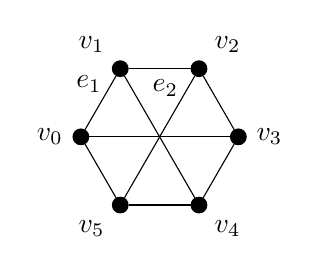
\begin{tikzpicture}[scale=1]
    \tikzstyle{v}=[draw, circle, minimum size=0.1cm, font=\footnotesize]
    \tikzstyle{c}=[draw, circle, inner sep=2, fill=black]
    \tikzstyle{e}=[]

    \node[c] (v0) at (  -1,  0)     [label=left:$v_0$]{};
    \node[c] (v1) at (-0.5,  0.866) [label=above left:$v_1$]{};
    \node[c] (v2) at ( 0.5,  0.866) [label=above right:$v_2$]{};
    \node[c] (v3) at (   1,  0)     [label=right:$v_3$]{};
    \node[c] (v4) at ( 0.5, -0.866) [label=below right:$v_4$]{};
    \node[c] (v5) at (-0.5, -0.866) [label=below left:$v_5$]{};

    \tedge{v3}{v2}{solid}{}{};
    \tedge{v2}{v1}{solid}{}{};
    \tedge{v1}{v0}{solid}{$e_1$}{left, pos=0.15};
    \tedge{v0}{v5}{solid}{}{};
    \tedge{v5}{v4}{solid}{}{};
    \tedge{v4}{v3}{solid}{}{};

    \tedge{v3}{v0}{solid}{}{};
    \tedge{v2}{v5}{solid}{$e_2$}{left, pos=0.1};
    \tedge{v1}{v4}{solid}{}{};
\end{tikzpicture}

    \caption{}\label{fig:omd_k33_example:a}
\end{subfigure}\hfill
\begin{subfigure}{.15\linewidth}\centering
    % \newcommand{\tedge}[5]{\draw[#3] (#1)-- node[e, #5] (e#4) {#4} (#2)}

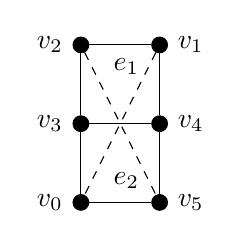
\begin{tikzpicture}[scale=1]
    \tikzstyle{v}=[draw, circle, minimum size=0.1cm, font=\footnotesize]
    \tikzstyle{c}=[draw, circle, inner sep=2, fill=black]
    \tikzstyle{e}=[]

    \node[c] (v0) at (0, 0) [label=left:$v_0$]{};
    \node[c] (v1) at (1, 2) [label=right:$v_1$]{};
    \node[c] (v2) at (0, 2) [label=left:$v_2$]{};
    \node[c] (v3) at (0, 1) [label=left:$v_3$]{};
    \node[c] (v4) at (1, 1) [label=right:$v_4$]{};
    \node[c] (v5) at (1, 0) [label=right:$v_5$]{};

    \tedge{v3}{v2}{solid}{}{};
    \tedge{v2}{v1}{solid}{}{};
    \tedge{v1}{v0}{dashed}{$e_1$}{left, pos=0.1};
    \tedge{v0}{v5}{solid}{}{};
    \tedge{v5}{v4}{solid}{}{};
    \tedge{v4}{v3}{solid}{}{};

    \tedge{v3}{v0}{solid}{}{};
    \tedge{v2}{v5}{dashed}{$e_2$}{left, pos=0.9};
    \tedge{v1}{v4}{solid}{}{};
\end{tikzpicture}

    \caption{}\label{fig:omd_k33_example:b}
\end{subfigure}
\begin{subfigure}{.15\linewidth}\centering
    % \newcommand{\tedge}[5]{\draw[#3] (#1)-- node[e, #5] (e#4) {#4} (#2)}

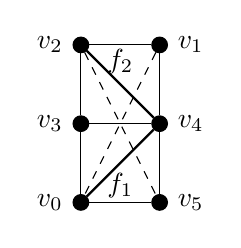
\begin{tikzpicture}[scale=1]
    \tikzstyle{v}=[draw, circle, minimum size=0.1cm, font=\footnotesize]
    \tikzstyle{c}=[draw, circle, inner sep=2, fill=black]
    \tikzstyle{e}=[]

    \node[c] (v0) at (0, 0) [label=left:$v_0$]{};
    \node[c] (v1) at (1, 2) [label=right:$v_1$]{};
    \node[c] (v2) at (0, 2) [label=left:$v_2$]{};
    \node[c] (v3) at (0, 1) [label=left:$v_3$]{};
    \node[c] (v4) at (1, 1) [label=right:$v_4$]{};
    \node[c] (v5) at (1, 0) [label=right:$v_5$]{};

    \tedge{v3}{v2}{solid}{}{};
    \tedge{v2}{v1}{solid}{}{};
    \tedge{v1}{v0}{dashed}{}{left, pos=0.15};
    \tedge{v0}{v5}{solid}{}{};
    \tedge{v5}{v4}{solid}{}{};
    \tedge{v4}{v3}{solid}{}{};

    \tedge{v3}{v0}{solid}{}{};
    \tedge{v2}{v5}{dashed}{}{left, pos=0.85};
    \tedge{v1}{v4}{solid}{}{};

    \tedge{v0}{v4}{solid, thick}{$f_1$}{below, pos=0.5};
    \tedge{v2}{v4}{solid, thick}{$f_2$}{above, pos=0.5};
\end{tikzpicture}

    \caption{}\label{fig:omd_k33_example:c}
\end{subfigure}\hfill
\begin{subfigure}{.15\linewidth}\centering
    % \newcommand{\tedge}[5]{\draw[#3] (#1)-- node[e, #5] (e#4) {#4} (#2)}

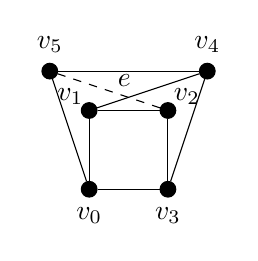
\begin{tikzpicture}
    \tikzstyle{v}=[draw, circle, minimum size=0.1cm, font=\footnotesize]
    \tikzstyle{c}=[draw, circle, inner sep=2, fill=black]
    \tikzstyle{e}=[]

    \node[c] (v0) at (  0,   0) [label=below:$v_0$]{};
    \node[c] (v1) at (  0,   1) [label={above left,inner sep=0pt,outer sep=0pt}:$v_1$]{};
    \node[c] (v2) at (  1,   1) [label={above right,inner sep=0pt,outer sep=0pt}:$v_2$]{};
    \node[c] (v3) at (  1,   0) [label=below:$v_3$]{};
    \node[c] (v4) at (1.5, 1.5) [label=above:$v_4$]{};
    \node[c] (v5) at (-.5, 1.5) [label=above:$v_5$]{};

    \tedge{v3}{v2}{solid}{}{};
    \tedge{v2}{v1}{solid}{}{};
    \tedge{v1}{v0}{solid}{}{};
    \tedge{v0}{v5}{solid}{}{};
    \tedge{v5}{v4}{solid}{}{};
    \tedge{v4}{v3}{solid}{}{};

    \tedge{v3}{v0}{solid}{}{};
    \tedge{v2}{v5}{dashed}{$e$}{above, pos=.35};
    \tedge{v1}{v4}{solid}{}{};
\end{tikzpicture}

    \caption{}\label{fig:omd_k33_example:d}
\end{subfigure}
\begin{subfigure}{.15\linewidth}\centering
    % \newcommand{\tedge}[5]{\draw[#3] (#1)-- node[e, #5] (e#4) {#4} (#2)}

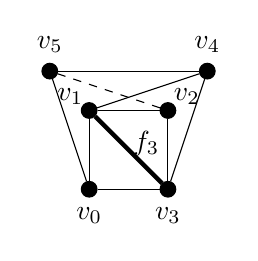
\begin{tikzpicture}
    \tikzstyle{v}=[draw, circle, minimum size=0.1cm, font=\footnotesize]
    \tikzstyle{c}=[draw, circle, inner sep=2, fill=black]
    \tikzstyle{e}=[]

    \node[c] (v0) at (  0,   0) [label=below:$v_0$]{};
    \node[c] (v1) at (  0,   1) [label={above left,inner sep=0pt,outer sep=0pt}:$v_1$]{};
    \node[c] (v2) at (  1,   1) [label={above right,inner sep=0pt,outer sep=0pt}:$v_2$]{};
    \node[c] (v3) at (  1,   0) [label=below:$v_3$]{};
    \node[c] (v4) at (1.5, 1.5) [label=above:$v_4$]{};
    \node[c] (v5) at (-.5, 1.5) [label=above:$v_5$]{};

    \tedge{v3}{v2}{solid}{}{};
    \tedge{v2}{v1}{solid}{}{};
    \tedge{v1}{v0}{solid}{}{};
    \tedge{v0}{v5}{solid}{}{};
    \tedge{v5}{v4}{solid}{}{};
    \tedge{v4}{v3}{solid}{}{};

    \tedge{v3}{v0}{solid}{}{};
    \tedge{v2}{v5}{dashed}{}{above, pos=.35};
    \tedge{v1}{v4}{solid}{}{};

    \tedge{v1}{v3}{solid, ultra thick}{$f_3$}{right, pos=0.4};
\end{tikzpicture}

    \caption{}\label{fig:omd_k33_example:e}
\end{subfigure}

\caption{
(\ref{fig:omd_k33_example:a}) The $K_{3,3}$ with two labeled edges, $e_1$ and $e_2$. (\ref{fig:omd_k33_example:b}) The $K_{3,3}$ with $e_1$ and $e_2$ removed (dashed lines) and rearranged to illustrate that it is now a partial 2-tree. (\ref{fig:omd_k33_example:c}) The $K_{3,3}$ with $\{e_1,e_2\}$ removed and $\{f_1,f_2\}$ (bold lines) added to make a 2-tree, showing that the $K_{3,3}$ is at least $OMD_2$. (\ref{fig:omd_k33_example:d}) The $K_{3,3}$ with only $e_2$ removed (dashed line). (\ref{fig:omd_k33_example:e}) The $K_{3,3}$ with $e_2$ removed and $f_3$ (bold line) added to make a low Cayley complexity graph, showing that the $K_{3,3}$ is $OMD_1$.
}
\label{fig:omd_k33_example}
\end{figure*}

\noindent
\note A huge advantage of the convex Cayley method is that it is
completely unaffected when $\delta$ are intervals rather than exact
values~\cite{sitharam2010convex}.

\myexample
A graph $G=K_{3,3}$  cannot be decomposed into any nontrivial
isostatic graphs, i.e, its DR-plan has a root and 9 children
corresponding to the 9 edges. Solving or recombining the system
$(G,\delta)$ corresponding to the root of this DR-plan involves
solving a quadratic system with 8 equations and variables. Instead of
simultaneously solving this system, we could instead use the fact that
$G=K_{3,3}$ is in OMD$_1$: remove the edge $e$ in Figure
\ref{fig:omd_k33_example} to give a partial 2-tree $G'$. Now add the
non-edge $f$ to give a 2-tree $H$ with a DR-plan of size 2. The Cayley
configuration space $\Phi_f(G', \delta_{E\setminus e})$ is a single
interval of attainable length values $\lambda_F$ for the edge $f$.
When $\delta$ is generic, i.e, does not admit collinearities or
coincidences in the realizations of $(G,\delta)$, the realization
space of $(H, \left<\delta_{E\setminus e}, \lambda_f\right>)$ has 16
solutions $q^p_{\lambda_f}$ (modulo orientation preserving
isometries), with distinct orientation types $\sigma_p$ (two
orientation choices for each of the 4 triangles) that can be obtained
by solving a sequence of 4 single quadratics in 1 variable (DR-plan of
size 2). By subdivided binary search in the interval $\lambda_f \in
\Phi_f(G', \delta_{E\setminus e})$, the desired solution $p$  of
$(G,\delta)$ is found when the length of the non-edge $e$ in  the
realization $q^p_{\lambda_f}$ is $\delta_e$.
%
\subsection{Optimized Modification by Enlarging the class of Reduced
Graphs}
\label{sec:tdecomp}
%
It is possible in principle to decrease $k$ for a OMD$_k$ graph (i.e,
the number of edges to be removed to ensure an isostatic completion
that is decomposable with a small DR-plan) by considering reduced
graphs $G'$ (and modified graphs $H$) that come from a larger class
than partial 2-trees but nevertheless have convex Cayley configuration
spaces at least when the realization space is restricted to a
sufficiently comprehensive orientation type. In particular, the so-
called \dfn{tree-decomposable graphs of low Cayley complexity}
\cite{sitharam2011cayleyI,sitharam2011cayleyII} include the partial 2-trees and many others that are not
partial 2-trees. These too result in DR-plans of size 2 or 3, putting
$G$ in the class OMD$_k$ and thus meeting Criteria (a) and (b). The
Criterion (c) is met --- for example when $k=1$ --- because 1-dof Cayley
configuration spaces of linkages based on such graphs $G'$ are known
to be single intervals when a comprehensive orientation type
$\sigma_p$ of the sought solution $p$ is given. In addition, the
bounds of these intervals are of low algebraic complexity. More
precisely, the bounds  can themselves be computed using a DR-plan of
size 2 or 3, i.e, the computation of these bounds is tree-
decomposable. Alternatively, the bounds are in a simple quadratic or
radically solvable extension field over the rationals, or can be
computed by solving a triangularized system of quadratics.

\section{Solution Space Navigation}

Discussion about software. Intuitive GUI that is \textit{essential} to the software and solving of the problem.


\section{Conclusion}

Wrap it up.



% \begin{figure}\centering
%   
\includegraphics[scale=.5]{example.eps}
%   \caption{Example of a normal figure that spans one column.}
%   \label{fig:square}
% \end{figure}

% \begin{figure*}\centering
%     
\includegraphics{example.eps}
%     \caption{Example of a figure that spans both columns.}
% \end{figure*}


%%%%%%%%%%%%%%%%%%%%%%%%%%%%%%%%%%%%%%%%%%%%%%%%%%%%%%%%%%%%%%%%%%%%

\bibliographystyle{abbrv}
\bibliography{paper}

\end{document}
